\documentclass{beamer}

%% \documentclass[handout]{beamer}
%% % use this with the [handout] option to create handouts for the audience
%% \usepackage{pgfpages}
%% \pgfpagesuselayout{2 on 1}[a4paper,border shrink=5mm]

\mode<presentation>
{
  \usetheme{Diku}
% set this to your preferences:
  \setbeamercovered{invisible}
%  \setbeamercovered{transparent}
}

\usepackage{graphicx}
\usepackage{epic}

\usepackage{amsmath}
\usepackage{amssymb}
\usepackage{amsthm}

\newcommand{\basetop}[1]{\vtop{\vskip-1ex\hbox{#1}}}
\newcommand{\source}[1]{\let\thefootnote\relax\footnotetext{\scriptsize\textcolor{kugray1}{Source: #1}}}

% for coloured code citation in text:
\usepackage{fancyvrb}

%%%%%%%%%%%%%%%%%%%%%%%%%%%%%%%%%
%%%%%    code sections   %%%%%%%%
%%%%%%%%%%%%%%%%%%%%%%%%%%%%%%%%%

% code highlighting commands in own block
\DefineVerbatimEnvironment{code}{Verbatim}{fontsize=\scriptsize}
\DefineVerbatimEnvironment{icode}{Verbatim}{fontsize=\scriptsize}

% Fancy code with color commands:
\DefineVerbatimEnvironment{colorcode}%
        {Verbatim}{fontsize=\scriptsize,commandchars=\\\{\}}

%%%%%%%%%%%%%%%%%%%%%%%%%%%%%%%%%%
%%%%%    some coloring    %%%%%%%%

\definecolor{Red}{RGB}{220,50,10}
\definecolor{Blue}{RGB}{0,51,102}
\definecolor{Yellow}{RGB}{102,51,0}
\definecolor{Orange}{RGB}{178,36,36}
\definecolor{Grey}{RGB}{180,180,180}
\definecolor{Green}{RGB}{20,120,20}
\definecolor{Purple}{RGB}{160,50,100}
\newcommand{\red}[1]{\textcolor{Red}{{#1}}}
\newcommand{\blue}[1]{\textcolor{Blue}{{#1}}}
\newcommand{\yellow}[1]{\textcolor{Yellow}{{#1}}}
\newcommand{\orange}[1]{\textcolor{Orange}{{#1}}}
\newcommand{\grey}[1]{\textcolor{Grey}{{#1}}}
\newcommand{\green}[1]{\textcolor{Green}{{#1}}}
\newcommand{\purple}[1]{\textcolor{Purple}{{#1}}}




% use "DIKU green" from our color theme for \emph
\renewcommand{\emph}[1]{\textcolor{structure}{#1}}
% use some not-too-bright red for an \emp command
\definecolor{DikuRed}{RGB}{130,50,32}
\newcommand{\emp}[1]{\textcolor{DikuRed}{ #1}}
\definecolor{CosGreen}{RGB}{10,100,70}
\newcommand{\emphh}[1]{\textcolor{CosGreen}{ #1}}
\definecolor{CosBlue}{RGB}{55,111,122}
\newcommand{\emphb}[1]{\textcolor{CosBlue}{ #1}}
\definecolor{CosRed}{RGB}{253,1,1}
\newcommand{\empr}[1]{\textcolor{CosRed}{ #1}}

\newcommand{\mymath}[1]{$ #1 $}
\newcommand{\myindx}[1]{_{#1}}
\newcommand{\myindu}[1]{^{#1}}

\newcommand{\Fasto}{\textsc{Fasto}\xspace}


%%%%%%%%%%%%%%%%%%%%

\title[VLIW Arch]{Optimizing Instruction-Level Parallelism ILP\\VLIW Architecture}

\author[C.~Oancea]{Cosmin E. Oancea\\{\tt cosmin.oancea@diku.dk}}

\institute{Department of Computer Science (DIKU)\\University of Copenhagen}

\date[Sept 2018]{September 2018 PMPH Lecture Slides}


\begin{document}

\titleslide

\begin{frame}
\frametitle{Structure of a Compiler}

\begin{tabular}{ccc}
Program text&&\\
$\downarrow$ &&\\
\framebox{Lexical analysis} && Binary machine code\\
$\downarrow$ && $\uparrow$ \\
Symbol sequence && \textcolor{gray}{\framebox{Assembly and linking}} \\
$\downarrow$ && $\uparrow$ \\
\framebox{Syntax analysis} && Ditto with named registers\\
$\downarrow$ && $\uparrow$ \\
\red{Syntax tree $\rightarrow$ \framebox{Intepretation}} && \framebox{Register allocation} \\
$\downarrow$ && $\uparrow$ \\
\framebox{Typecheck} && Symbolic machine code\\
$\downarrow$ &&  $\uparrow$ \\
Syntax tree  && \framebox{Machine code generation} \\
$\downarrow$ && $\uparrow$ \\
\framebox{Intermediate code generation} &$\longrightarrow$ & Intermediate code
\end{tabular}

\end{frame}


\begin{frame}
\frametitle{Acknowledgments}
This lecture presents selected Topics from Chapter 3 of the\\
``Parallel Computer Organization and Design`` book,\\
by Michel Dubois, Murali Annavaram and Per Stenstrom.
\end{frame}


\begin{frame}[fragile]
	\tableofcontents
\end{frame}


%%%%%%%%%%%%%%%%%%%%%%%%%%%%%%%%%%%%%%%%%%%%%%%%%%%%%%%%%%%%%%%%%%%%%%
%%%%%%%%%%%%%%%%%%%%%%%%%%%%%%%%%%%%%%%%%%%%%%%%%%%%%%%%%%%%%%%%%%%%%%
%%%%%%%%%%%%%%%%%%%%%%%%%%%%%%%%%%%%%%%%%%%%%%%%%%%%%%%%%%%%%%%%%%%%%%
\section{Instruction-Scheduling for ILP}


\begin{frame}[fragile,t]
\frametitle{Instruction Scheduling}

\begin{itemize}
    \item {Dynamic} by hardware: the ever-wider dispatch width
            $\Rightarrow$ 
            more \& more complex, slower, and power-hungry hardware. \smallskip
 
    \item {\em Static} by compiler: instruction reordering aimed at
            minimizing the number of stalls,
            e.g., linear pipeline, superpipeline, superscalar, VLIW.  
\end  {itemize}
\pause\bigskip

Compiler has a better structural view of the entire code, but has less reliable info 
@ execution time than hardware. Code Motion:
\smallskip
\begin{itemize}
    \item \emph{\em Local}, i.e., within a \alert{basic block (BB)?}. 
    \item \emph{\em Global} (across BBs): 
    \begin{itemize}
        \item \emp{\em cyclic}, meaning on \alert{loops?}, e.g., loop unrolling, software pipelining.
        \item \emp{\em non-cyclic}, e.g., trace scheduling: schedule issued for the most likely 
                program trace based on static prediction (profiling) + compensation code 
                for all other possible traces.
    \end  {itemize}
\end  {itemize}

\end{frame}

\subsection{Local Scheduling: Simple Code Motion}

\begin{frame}[fragile,t]
    \frametitle{Local Scheduling: Code Motion In a Basic Block}

\begin{block}{HL Code{\tt~~~~~~~~}Unoptimized}\vspace{-2ex}
\begin{columns}
\column{0.18\textwidth}
\begin{colorcode}[fontsize=\scriptsize]
for(i=0;i<100;i++)
  A[i]=A[i]+B[i]
\end{colorcode} 
\column{0.40\textwidth}
\begin{colorcode}[fontsize=\scriptsize]
//R3=100, R1/2=@A/B 
Loop: L.S   F0, 0(R1)   (1)
      L.S   F1, 0(R2)   (1)
      ADD.S F2, F1, F0  (2)
      S.S   F2, 0(R1)   (5)
      ADDI  R1, R1, #4  (1)
      ADDI  R2, R2, #4  (1)
      SUBI  R3, R3, #1  (1)
      BNEZ  R3, Loop    (3)
\end{colorcode} 
\column{0.40\textwidth}
\begin{colorcode}[fontsize=\scriptsize]

\end{colorcode} 
\end{columns}
\end{block}

\bigskip
\bigskip

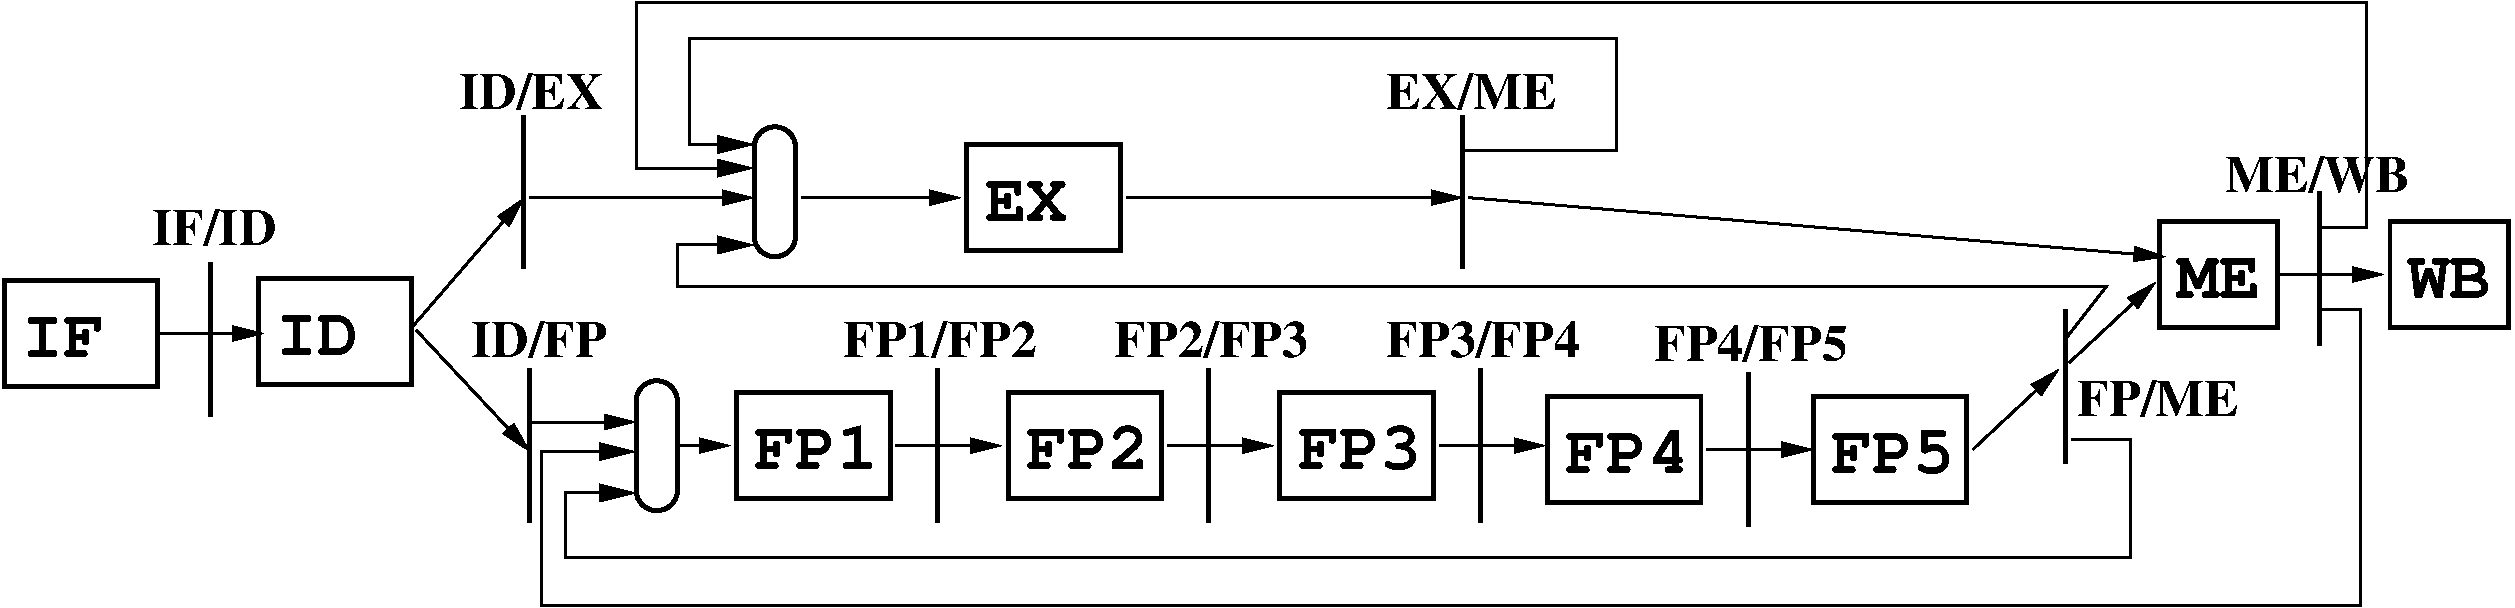
\includegraphics[width=53ex]{Figures/SimpleOoOPipeline}

\end{frame}


\begin{frame}[fragile,t]
    \frametitle{Local Scheduling: Code Motion In a Basic Block}

\begin{block}{HL Code{\tt~~~~~~~~}Unoptimized}\vspace{-2ex}
\begin{columns}
\column{0.18\textwidth}
\begin{colorcode}[fontsize=\scriptsize]
for(i=0;i<100;i++)
  A[i]=A[i]+B[i]
\end{colorcode} 
\column{0.40\textwidth}
\begin{colorcode}[fontsize=\scriptsize]
//R3=100, R1/2=@A/B 
Loop: L.S   F0, 0(R1)   (1)
      L.S   F1, 0(R2)   (1)
      ADD.S F2, F1, F0  (2)
      S.S   F2, 0(R1)   (5)
      ADDI  R1, R1, #4  (1)
      ADDI  R2, R2, #4  (1)
      SUBI  R3, R3, #1  (1)
      BNEZ  R3, Loop    (3)
\end{colorcode} 
\column{0.40\textwidth}
\begin{colorcode}[fontsize=\scriptsize]

\end{colorcode} 
\end{columns}
\end{block}

In parenthesis is shown \# of clocks taken by each instr
in a single-issue static pipeline with separate integer an float 
execution:\smallskip
\begin{itemize}
    \item {\em branch}: 1 if untaken, 3 if taken (2 instr are flushed) $\Rightarrow$ 
            move it to the top of the loop.\\  
            \emp{\bf Delayed branches (ISA extension): put two instrs
            after the branch to be executed regardless of the branch.}
    \item {\em other}: \# cycles spent in ID stage due to data-hazards stalls,
    \item Unoptimized code \#clocks = 15.
\end  {itemize}

\end{frame}

\begin{frame}[fragile,t]
    \frametitle{Local Scheduling: Code Motion In a Basic Block}

\begin{block}{HL Code{\tt~~~~~~~~}Unoptimized{\tt~~~~~~~~~}After Code Motion}\vspace{-2ex}
\begin{columns}
\column{0.18\textwidth}
\begin{colorcode}[fontsize=\scriptsize]
for(i=0;i<100;i++)
  A[i]=A[i]+B[i]
\end{colorcode} 
\column{0.40\textwidth}
\begin{colorcode}[fontsize=\scriptsize]
//R3=100, R1/2=@A/B 
Loop: L.S   F0, 0(R1)   (1)
      L.S   F1, 0(R2)   (1)
      ADD.S F2, F1, F0  (2)
      S.S   F2, 0(R1)   (5)
      ADDI  R1, R1, #4  (1)
      ADDI  R2, R2, #4  (1)
      SUBI  R3, R3, #1  (1)
      BNEZ  R3, Loop    (3)
\end{colorcode} 
\column{0.40\textwidth}
\begin{colorcode}[fontsize=\scriptsize]
//R3=100, R1/2=@A/B 
Loop: L.S   F0, 0(R1)   (1)
      L.S   F1, 0(R2)   (1)
      \emp{SUBI  R3, R3, #1  (1)}    
      ADD.S F2, F1, F0  (1)
      ADDI  R1, R1, #4  (1)
      ADDI  R2, R2, #4  (1)
      \emp{S.S   F2, -4(R1)  (3)}
      BNEZ  R3, Loop    (3)
\end{colorcode} 
\end{columns}
\end{block}

In parenthesis is shown \# of clocks taken by each instr
in a single-issue static pipeline with separate integer an float 
execution:\smallskip
\begin{itemize}
    \item {\tt SUB.I} \emp{moved up} after {\tt L.S} to eliminate the stall
            caused by a load followed by a dependent use. 
    \item {S.S} \emp{moved down} far away from the {ADD.S} it depends on, but
    \item introduces {\sc WAR} dependency, solved by adjusting {\tt S.S}'s 
            displ. 
\end  {itemize}

\emph{Unoptim\#clocks = 15, Optimized\#clocks = 12, Speedup = 1.25$\times$.}

\end{frame}

\subsection{Cyclic Scheduling: Loop Unrolling}
\begin{frame}[fragile,t]
    \frametitle{Loop Unrolling}

Basic Blocks have on average 4-5 instructions $\Rightarrow$ limited benefits.
\smallskip

Loop Unrolling: schedules computed across several iterations.

\begin{block}{Original{\tt~~~~~~~~}Unroll Twice{\tt~~~}Rename Registers{\tt~~}Loads$\uparrow$ Stores$\downarrow$}\vspace{-2ex}
\begin{columns}
\column{0.22\textwidth}
\begin{colorcode}[fontsize=\scriptsize]
for(i=0;i<100;i++)
  t1 = A[i]
  t2 = B[i]
  t3 = t1+t2
  A[i] = t3
\end{colorcode} 
\column{0.24\textwidth}
\begin{colorcode}[fontsize=\scriptsize]
for(i=0;i<100;i+=2)
  t1 = A[i]
  t2 = B[i]
  t3 = t1+t2
  A[i] = t3
  \emp{t1 = A[i+1]}
  \emp{t2 = B[i+1]}
  \emp{t3 = t1+t2}
  \emp{A[i+1] = t3}
\end{colorcode} 
\column{0.24\textwidth}
\begin{colorcode}[fontsize=\scriptsize]
for(i=0;i<100;i+=2)
  t1 = A[i]
  t2 = B[i]
  t3 = t1+t2
  A[i] = t3
  \emph{t4} = A[i+1]
  \emph{t5} = B[i+1]
  \emph{t6} = t4+t5
  A[i+1] = \emph{t6}
\end{colorcode} 
\column{0.24\textwidth}
\begin{colorcode}[fontsize=\scriptsize]
for(i=0;i<100;i+=2)
  t1 = \emph{A[i]}
  t2 = \emph{B[i]}
  t4 = \emph{A[i+1]}
  t5 = \emph{B[i+1]}
  t3 = t1+t2
  t6 = t4+t5
  \emp{A[i]} = t3
  \emp{A[i+1]} = t6
\end{colorcode} 
\end{columns}
\end{block}
\smallskip \pause

With our example {\tt for(i=0;i<100;i++) A[i]+=B[i]} in {\sc tac} form:
\begin{itemize}
    \item unroll twice, but epilog is required if unknown loop count,
    \item code motion in the expanded body limited by WAW, WAR deps,
    \item which are fixed by {\bf \emph{renaming}} registers \& adjusting displacements,
    \item finally, loads are moved up and stores down
\end{itemize}

\end{frame}

\begin{frame}[fragile,t]
    \frametitle{Loop Unrolling on A Single-Issue Pipeline}

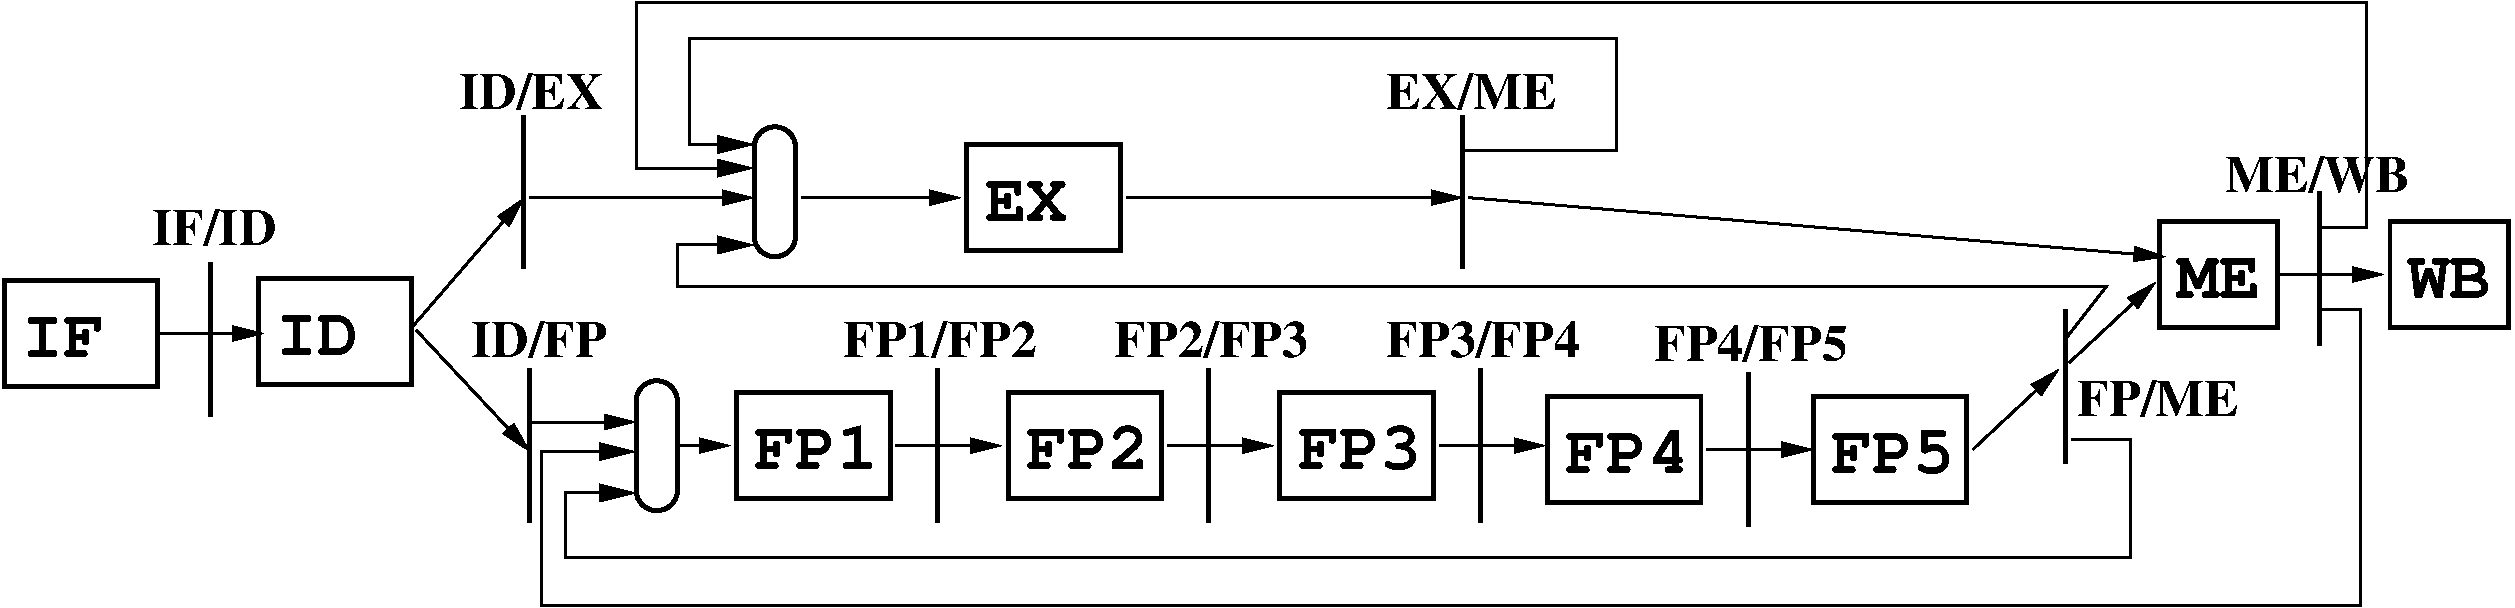
\includegraphics[width=50ex]{Figures/SimpleOoOPipeline}

\begin{block}{TAC Optim Code{\tt~~~~~~~~~~~}MIPS Optim Code~~~~~~\# clocks in ID}\vspace{-2ex}
\begin{columns}
\column{0.42\textwidth}
\begin{colorcode}[fontsize=\scriptsize]
for(i=0;i<100;i+=2)
  t1 = \emph{A[i]}
  t2 = \emph{B[i]}
  t4 = \emph{A[i+1]}
  t5 = \emph{B[i+1]}
  t3 = t1+t2
  t6 = t4+t5
  \emp{A[i]} = t3
  \emp{A[i+1]} = t6
\end{colorcode}
\column{0.55\textwidth}
\begin{colorcode}[fontsize=\scriptsize]
Loop: \emph{L.S   F0, 0(R1)}   (1)
      \emph{L.S   F1, 0(R2)}   (1) 
      \emph{L.S   F3, 4(R1)}   (1)
      \emph{L.S   F4, 4(R2)}   (1)
      ADD.S F2, F1, F0  (1)
      ADD.S F5, F3, F4  (1)
      SUBI  R3, R3, #2  (1)
      ADDI  R1, R1, #8  (1)
      ADDI  R2, R2, #8  (1)
      \emp{S.S   F2, -8(R1)}  (1)
      \emp{S.S   F5, -4(R1)}  (1)
      BNEZ  R3, Loop    (3)
\end{colorcode}  
\end{columns}
\end{block}
\smallskip 

\# clocks for 2 iters: 14 $\Rightarrow$ Speedup = 15/7 = 2.14$\times$

\end{frame}


\begin{frame}[fragile,t]
    \frametitle{Loop Unrolling on A 5-stage-FP-Unit Super-Pipeline}

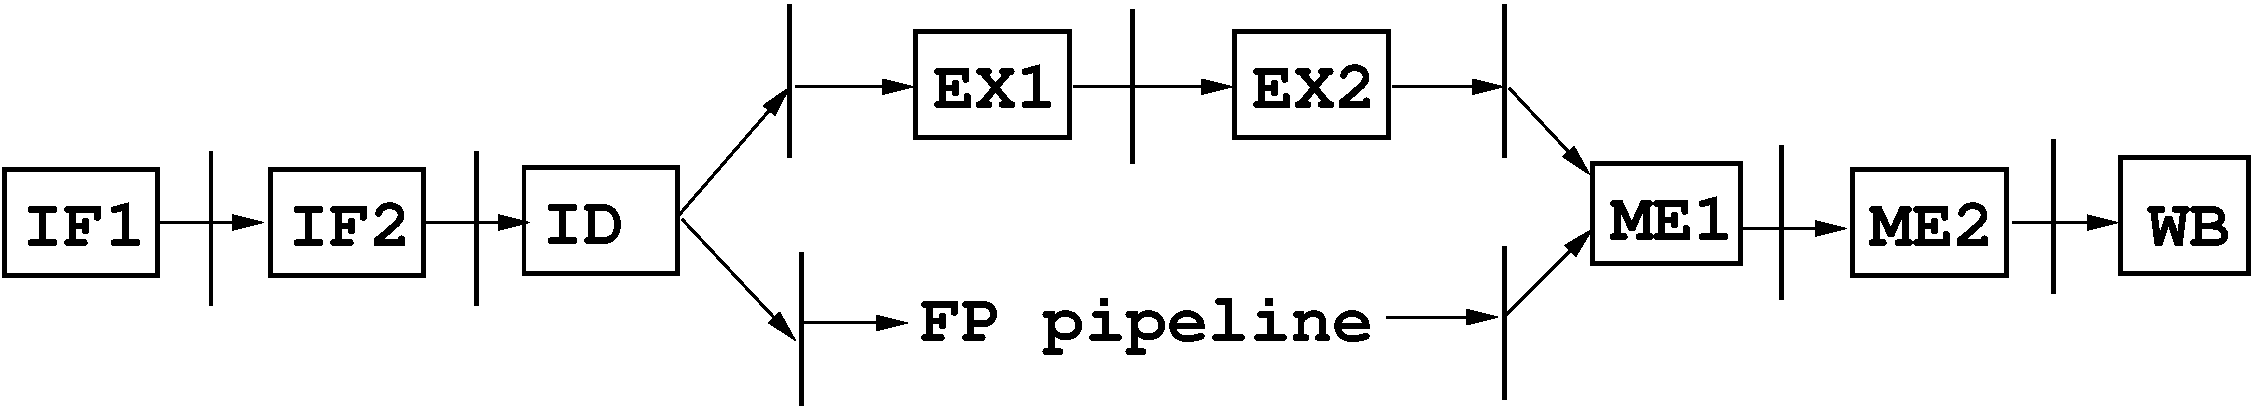
\includegraphics[width=50ex]{Figures/SuperPipeline}

\begin{block}{TAC Optim Code{\tt~~~~~~~~~~~}MIPS Optim Code~~~~~~\# clocks in ID}\vspace{-2ex}
\begin{columns}
\column{0.42\textwidth}
\begin{colorcode}[fontsize=\scriptsize]
for(i=0;i<100;i+=2)
  t1 = \emph{A[i]}
  t2 = \emph{B[i]}
  t4 = \emph{A[i+1]}
  t5 = \emph{B[i+1]}
  t3 = t1+t2
  t6 = t4+t5
  \emp{A[i]} = t3
  \emp{A[i+1]} = t6
\end{colorcode}
\column{0.55\textwidth}
\begin{colorcode}[fontsize=\scriptsize]
Loop: \emph{L.S   F0, 0(R1)}   (1)
      \emph{L.S   F1, 0(R2)}   (1) 
      \emph{L.S   F3, 4(R1)}   (1)
      \emph{L.S   F4, 4(R2)}   (1)
      ADD.S F2, F1, F0  (2)
      ADD.S F5, F3, F4  (2)
      SUBI  R3, R3, #2  (1)
      ADDI  R1, R1, #8  (1)
      ADDI  R2, R2, #8  (1)
      \emp{S.S   F2, -8(R1)}  (1)
      \emp{S.S   F5, -4(R1)}  (1)
      BNEZ  R3, Loop    (4)
\end{colorcode}  
\end{columns}
\end{block}
\smallskip 

17 clocks for 2 iters, or 8.5 clocks per iteration, but the clock rate 
is twice as fast $\Rightarrow$ Speedup = 2*15/8.5 = 3.52$\times$.

\end{frame}

\begin{frame}[fragile,t]
    \frametitle{Loop Unrolling on A Super-Scalar}

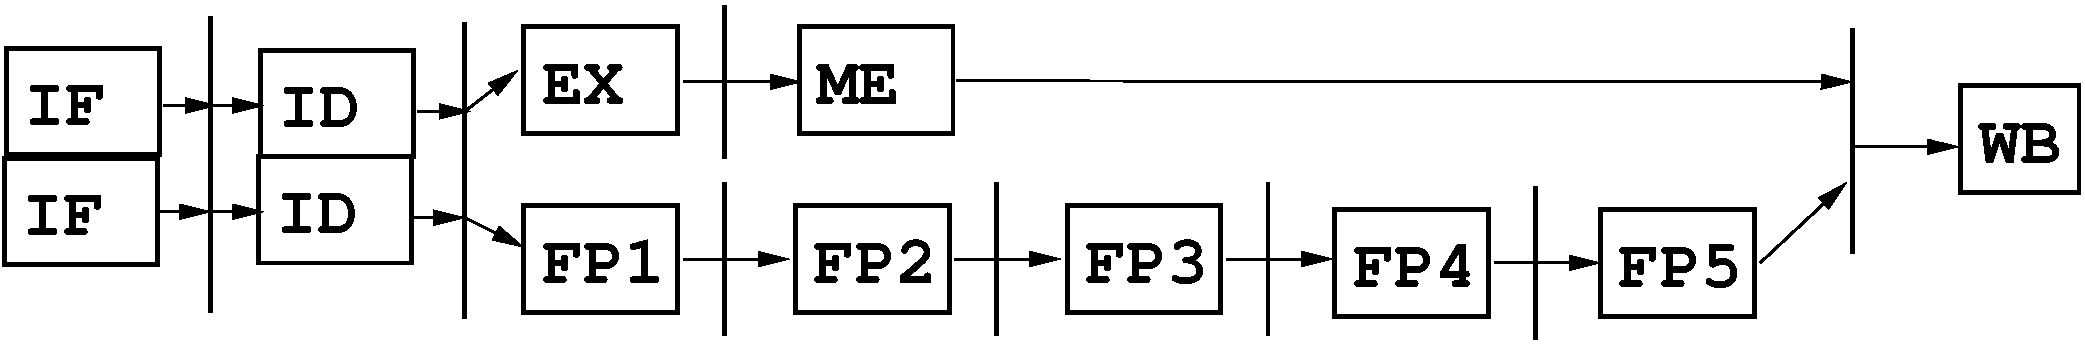
\includegraphics[width=33ex]{Figures/SuperScalar}

Modest speedup $2.14\times$ because fraction of FP instrs is small:
%Does not fare well because the fraction of FP instrs is small:\\
%14 cycles for 2 iters $\Rightarrow$ Speedup = 15/7 = 2.14$\times$

\begin{block}{TAC Optim Code{\tt~~~~~~~~~~~}MIPS Optim Code~~~~~~\# clocks in ID}\vspace{-2ex}
\begin{columns}
\column{0.25\textwidth}
\begin{colorcode}[fontsize=\scriptsize]
for(i=0;i<100;i+=2)
  t1 = \emph{A[i]}
  t2 = \emph{B[i]}
  t4 = \emph{A[i+1]}
  t5 = \emph{B[i+1]}
  t3 = t1+t2
  t6 = t4+t5
  \emp{A[i]} = t3
  \emp{A[i+1]} = t6
\end{colorcode}
\column{0.70\textwidth}
\begin{colorcode}[fontsize=\scriptsize]
Loop: \emph{L.S   F0, 0(R1)}                         (1)
      \emph{L.S   F1, 0(R2)}                         (1) 
      \emph{L.S   F3, 4(R1)}                         (1)
      \emph{L.S   F4, 4(R2)}                         (1)          
      SUBI  R3, R3, #2      ADD.S F2, F1, F0  (1)
      ADDI  R1, R1, #8      ADD.S F5, F3, F4  (1)
      ADDI  R2, R2, #8                        (1)
      \emp{S.S   F2, -8(R1)}                        (3)
      \emp{S.S   F5, -4(R1)}                        (1)
      BNEZ  R3, Loop                          (3)
\end{colorcode}  
\end{columns}
\end{block}
\smallskip

\emp{\bf Drawbacks of Loop Unrolling:}\pause
\begin{itemize}
    \item Ineffective for loop-carried dependencies (restrict code motion),
    \item Consumes many addressable registers (since renaming is critical),
    \item High code expansion of the loop body.
\end  {itemize}

\end{frame}

\subsection{Cyclic Scheduling: Software Pipelining}

\begin{frame}[fragile,t]
    \frametitle{Software Pipelining: Intuition}

Original loop ({\tt Orig\_It1-4}) transformed into another loop ({\tt P\_It1-3})
which {\em pipelines} the original's dependent instrs across multiple iters:

\bigskip

\begin{scriptsize}
\begin{tabular}{lllll}
\hline
        & Orig\_It1       & Orig\_It2      & Orig\_It3 & Orig\_It4 \\\hline
Prolog  & L.S F0, 0(R1)   & -               & -     & - \\
        & L.S F1, 0(R2)   &                 &       &   \\
        & ADD.S F2,F1,F0  &                 &       &   \\\hline
P\_It1  & S.S F2, 0(R1)   & L.S F0, 0(R1)   & -     & - \\
        &                 & L.S F1, 0(R2)   &       &    \\
        &                 & ADD.S F2,F1,F0  &       &    \\\hline
P\_It2  &                 & S.S F2, 0(R1)   & L.S F0, 0(R1)   & - \\
        &                 &                 & L.S F1, 0(R2)   &   \\
        &                 &                 & ADD.S F2,F1,F0  &   \\\hline
P\_It3  &                 &                 & S.S F2, 0(R1)   & L.S F0, 0(R1)  \\
        &                 &                 &                 & L.S F1, 0(R2)  \\
        &                 &                 &                 & ADD.S F2,F1,F0 \\\hline
Epilog  &                 &                 &                 & S.S F2, 0(R1)  \\\hline

\end{tabular}
\end{scriptsize}

Transformed code: {\tt prolog; pipelined\_loop; epilog;}\\
The order in which instrs are executed is the same row and column-wise.

\end{frame}

\begin{frame}[fragile,t]
    \frametitle{Software Pipelining Schedule}

\begin{block}{Local Optimized Code{\tt~~~~~~~~~~~~~~~}Pipelined Schedule:}\vspace{-2ex}
\begin{columns}
\column{0.60\textwidth}
\begin{colorcode}[fontsize=\scriptsize]
for(i=0;i<100;i++)
  A[i]=A[i]+B[i]

Loop: L.S   F0, 0(R1)   (1)
      L.S   F1, 0(R2)   (1)
      SUBI  R3, R3, #1  (1)
      ADD.S F2, F1, F0  (1)
      ADDI  R1, R1, #4  (1)
      ADDI  R2, R2, #4  (1)
      \emp{S.S   F2, -4(R1)  (3)}
      BNEZ  R3, Loop    (3)
\end{colorcode}
\begin{scriptsize}
\begin{itemize}
\item \emph{Avoids stalls without using more registers.}
\item \emph{Pipelined loop same size as original loop.}
\item \emph{Effective even when loop carries dependencies.}
\end{itemize}
\end{scriptsize}
\column{0.38\textwidth}
\begin{colorcode}[fontsize=\scriptsize]
Prolog: L.S   F0,0(R1)
        L.S   F1,0(R2)
        SUBI  R3,R3,#1
        ADD.S F2,F1,F0
        ADDI  R1,R1,#4
        ADDI  R2,R2,#4
Loop:   \emph{S.S   F2,-4(R1) (1)}
        L.S   F0,0(R1)  (1)
        L.S   F1,0(R2)  (1)
        SUBI  R3,R3,#1  (1)
        ADD.S F2,F1,F0  (1)
        ADDI  R1,R1,#4  (1)
        ADDI  R2,R2,#4  (1)
        BNEZ  R3, Loop  (3)
Epilog: S.S   F2,-4(R1)
\end{colorcode}
\end{columns}
\end{block}
\smallskip

\emp{Initiation Interval}: after how many clocks can a new (orig) iter start 
(concurrently with previous ones), such that latencies are respected?\\
\emph{In this case 3 cycles}: moving \emp{S.S} across exploits BNEZ latency. 

\end{frame}


\begin{frame}[fragile,t]
    \frametitle{Software Pipelining on Independent Loops}

The pipelined-loop iteration contains the same instructions 
but each corresponds to a different iteration of the original loop.

\begin{scriptsize}
\begin{itemize}
\item Assume Intra-Iteration Producer-Consumer Relation 
\begin{scriptsize}{\tt A(i)$\Rightarrow$B(i)$\Rightarrow\ldots \Rightarrow$F(i)}\end{scriptsize}
%$C(i)$\Rightarrow$D(i)$\Rightarrow$E(i)$
\item NO Cross-Iteration dependencies ({\tt A(i+1)} does not depend on {\tt B(i)}),
\end{itemize}
\end{scriptsize}


\begin{block}{Original{\tt~~~~}Pipelined{\tt~~~~~~~}Original/Pipeline=Columns/Rows}\vspace{-2ex}
\begin{columns}
\column{0.17\textwidth}
\begin{colorcode}[fontsize=\tiny]
for(i=1;i<=N;i++)
  A(i) // (3 cycle)
  B(i) // (3)
  C(i) // (3)
  D(i) // (12)
  E(i) // (3)
  F(i) // (3)
end
\end{colorcode}
\column{0.17\textwidth}
\begin{colorcode}[fontsize=\tiny]
prologue
for(i=1;i<=N-6;i++)
  A(i+6)
  B(i+5)
  C(i+4)
  D(i+2) //\alert{skip i+3}
  E(i+1)
  F(i)
end
epilogue
\end{colorcode}
\column{0.59\textwidth}\pause
\begin{colorcode}[fontsize=\tiny]
\emp{A(1)}                                      // \emp{prolog begins}
\emp{A(2), B(1)} 
\emp{A(3), B(2), C(1)} 
\emp{A(4), B(3), C(2)} 
\emp{A(5), B(4), C(3),     , D(1)}
\emp{A(6), B(5), C(4),     , D(2), E(1)} // \emph{loop begins}
\emph{A(7), B(6), C(5),     , D(3), E(2), F(1)   //It1}
\emph{A(8), B(7), C(6),     , D(4), E(3), F(2)   //It2}
\emph{A(9), B(8), C(7),     , D(5), E(4), F(3)   //It3}
\emp{.....                                     // epilogue begins} 
\end{colorcode}
\end{columns}
\end{block}
\smallskip

%\begin{scriptsize}
%\end{scriptsize}

\begin{scriptsize}
\begin{itemize}
\item \emph{Latencies Resolved: 7 instrs between A(7) and B(7), 12 between C(5) and D(5)} \pause
\item Loop Unrolling needs a factor 12$\times$ $\Rightarrow$ register \& cache pressure,
\item Soft Pipelining may require hardware support (\emp{rotating registers bank}) to fix
        WAR deps, and needs prolog and epilog code.
\item All stalls have been eliminated \& Each instruction {\tt A(i)$\ldots$F(i)} takes one clock and  
\item \emph{Apply first {\em loop unrolling}, and then {\em softw pipelining} 
        (because the latter introduces loop-carried dependencies!)}
\end{itemize}
\end{scriptsize}


\end{frame}


%%%%%%%%%%%%%%%%%%%%%%%%%%%%%%%%%%%%%%%%%%%%%%%%%%%%%
%%%%%%%%%%%%%%%%%%%%%%%%%%%%%%%%%%%%%%%%%%%%%%%%%%%%%
%%%%%%%%%%%%%%%%%%%%%%%%%%%%%%%%%%%%%%%%%%%%%%%%%%%%%

\section{Case Study: VLIW Architecture}

\begin{frame}[fragile]
	\tableofcontents[currentsection]
\end{frame}

\subsection{Architectural View}

\begin{frame}[fragile,t]
\frametitle{VLIW: Birds Eye View}

{\bf Very Long Instruction Word (VLIW)}: statically scheduled microarchitectures, 
        in which each (very) long instruction contains several MIPS instrs, 
        called ``{\sc ops}''.
    The {\sc ops} of the current LIW:\smallskip
\begin{itemize}
    \item are fetched at once, are decoded in parallel and 
    \item are applied each to a different pipeline (with optimized decoding)
    \item correspond to independent instructions
\end  {itemize}
\bigskip

%All hazards are solved by compiler:
%\begin{itemize}
%    \item WAW \& WAR solved by renaming registers
%    \item RAW \& structural \& control hazards are avoided by scheduling
%    \item exceptions or indirect memory accesses solved via dispatch codes.
%\end  {itemize}

\smallskip

%If enough ILP $\Rightarrow$ no blocking. All hazards are solved by compiler.\\
%
Minimizes hwd complexity and power \& enable
    superscalar arch with very-wide fetch and dispatch bandwidth.
All hazards solved by compiler; if enough exploitable ILP $\Rightarrow$ no stalls:\pause
\begin{itemize}
    \item RAW on registers: solved by inserting enough instrs (cycles) 
            between the source and destination of the dependency,\smallskip
    \item WAR and WAW solved by renaming registers,
    \item structural \& control hazards are avoided (by code scheduling),
    \item exceptions \& indirect mem access: speculative mechanisms relying on
             patch-up code to cancel unwanted execution results.  
\end  {itemize}


\end{frame}


\begin{frame}[fragile,t]
\frametitle{VLIW Architecture}

\begin{columns}
\column{0.55\textwidth}
\begin{scriptsize}
\begin{tabular}{ccccc}
\hline
MemOp1 & MemOp2 & FOp1 & FOp2 & Int/Branch \\\hline
$\downarrow$  & $\downarrow$  & $\downarrow$  & $\downarrow$  & $\downarrow$ \\
\framebox{ID} & \framebox{ID} & \framebox{ID} & \framebox{ID} & \framebox{ID} \\
$\downarrow$  & $\downarrow$  & $\downarrow$  & $\downarrow$  & $\downarrow$  \\
\framebox{EX} & \framebox{EX} & \framebox{EX} & \framebox{EX} & \framebox{EX} \\
$\downarrow$  & $\downarrow$  & $\downarrow$  & $\downarrow$  & $\downarrow$  \\
\framebox{ME} & \framebox{ME} & \framebox{EX} & \framebox{EX} & \framebox{WB} \\
$\downarrow$  & $\downarrow$  & $\downarrow$  & $\downarrow$  &               \\
\framebox{WB} & \framebox{WB} & \framebox{EX} & \framebox{EX} &               \\
              &               & $\downarrow$  & $\downarrow$  &               \\
              &               & \framebox{WB} & \framebox{WB} &               
\end{tabular}
\end{scriptsize}
\column{0.42\textwidth}
\begin{scriptsize}
\emp{~~~~~Operation Latencies For Various}\\
\emp{~~~~~ Forwarding (F) Assumptions:}\\
\begin{tabular}{|c|c|c|c|c|}
\hline
Source & Dest & NoF & RegF & FullF\\\hline
{\sc load}   & any  & 3     & 2      & 1      \\\hline
{\sc int}    & any  & 2     & 1      & 0      \\\hline
{\sc float}  & any  & 4     & 3      & 2      \\\hline
{\sc store}  & {\sc load} & 0     & 0      & 0      \\\hline
\end{tabular}  
\smallskip

Uses \emp{delayed branches} by 2 instrs to\\avoid flushing (simplest solution)!
\end{scriptsize}
\end{columns}

\pause\smallskip

Compiler needs to know the operation latency of each instruction:\\
\begin{itemize}
    \item without forwarding (NoF) instr cannot be scheduled before its parent (source) 
            {\bf has passed} the WB stage.
    \item with register forwarding (RegF) a value written in the WB stage is forwarded
            {\bf in the same cycle} to the (child) ID stage. 
    \item with full forwarding (FullF) instruction can be scheduled {\bf as soon as} 
            the result is available (in EX or ME).
\end  {itemize}

\end{frame}

\subsection{Code Example: Loop Unrolling \& Software Pipelining}

\begin{frame}[fragile,t]
    \frametitle{VLIW: Code Example}

\begin{colorcode}[fontsize=\scriptsize]
for(i=1000;i>0;i--)        Loop: L.D   F0, 0(R1)
  x[i] = x[i] + s                ADD.D F4, F0, F2
                                 S.D   F4, 0(R1)   
                                 SUBI  R1, R1, #8
                                 BNE   R1, R2, Loop
\end{colorcode}

\begin{tiny}
\begin{tabular}{llllll}
\hline
Clock   & MemOp1          & MemOp2 & FOp1  & FOp2 & Int/Branch    \\\hline
1       & L.D   F0, 0(R1) & NOOP   & NOOP  & NOOP & NOOP \\
2       & NOOP            & NOOP   & NOOP  & NOOP & SUBI R1,R1,\#8\\
3       & NOOP            & NOOP   & ADD.D F4,F0,F2  & NOOP & NOOP\\
4       & NOOP            & NOOP   & NOOP  & NOOP & BNE R1,R2,Loop\\
5       & NOOP            & NOOP   & NOOP  & NOOP & NOOP\\
6       & S.D F4, 8(R1)   & NOOP   & NOOP  & NOOP & NOOP\\\hline
\end{tabular}
\end{tiny}

\smallskip
\pause 

\begin{itemize}
    \item one instr needs to be inserted between L.D (load)
            and the dependent ADD.D
    \item two instructions need to be inserted between ADD.D
            and the dependent S.D (store).
    \item branches are delayed, i.e., two instructions inserted
            after BNE which semantically execute before BNE.
    \item without cyclic optimizations $\Rightarrow$ \alert{6 clocks/iteration (Terrible)}.
\end  {itemize}

\end{frame}


\begin{frame}[fragile,t]
    \frametitle{Schedule With Loop Unrolling}

\begin{colorcode}[fontsize=\scriptsize]
for(i=1000;i>0;i--)        Loop: L.D   F0, 0(R1)
  x[i] = x[i] + s                ADD.D F4, F0, F2
                                 S.D   F4, 0(R1)   
                                 SUBI  R1, R1, #8
                                 BNE   R1, R2, Loop
\end{colorcode}

\begin{tiny}
\begin{tabular}{llllll}
\hline
Clock   & MemOp1         & MemOp2         & FOp1            & FOp2             & Int/Branch \\\hline
1       & L.D F0,   0(R1)& L.D F6, - 8(R1)& NOOP            & NOOP             & NOOP \\
2       & L.D F10,-16(R1)& L.D F14,-24(R1)& NOOP            & NOOP             & NOOP \\
3       & L.D F18,-32(R1)& L.D F22,-40(R1)& ADD.D F4, F0, F2& ADD.D F8, F6, F2 & NOOP \\
4       & L.D F26,-48(R1)& NOOP           & ADD.D F12,F10,F2& ADD.D F16,F14,F2 & NOOP \\
5       & NOOP           & NOOP           & ADD.D F20,F18,F2& ADD.D F24,F22,F2 & NOOP\\
6       & S.D F4,  0(R1) & S.D F8, -8(R1) & ADD.D F28,F26,F2& NOOP             & SUBI R1,R1,\#56\\
7       & S.D F12,40(R1) & S.D F16,32(R1) & NOOP            & NOOP             & DBNE R1,R2,Loop\\
8       & S.D F20,24(R1) & S.D F24,16(R1) & NOOP            & NOOP             & NOOP\\
9       & S.D F28, 8(R1) & NOOP           & NOOP            & NOOP             & NOOP\\\hline
\end{tabular}
\end{tiny}

\smallskip

\begin{itemize}
    \item original loop was unrolled 7 times,
    \item register renaming and adjusting load/store displacements fixed WAR and WAW dependencies,
    \item \emp{code size of the loop increases $\sim7\times$, \& high register pressure,} 
    \item \emph{but schedule executes $7$ original-loop iterations in $9$ clocks, while
            respecting all dependencies. Speedup = 6*7 / 9 = 4.67$\times$}
\end  {itemize}

\end{frame}

\begin{frame}[fragile,t]
    \frametitle{Schedule With Software Pipelining}

\begin{colorcode}[fontsize=\tiny]
for(i=1000;i>0;i--)        Loop: L.D   F0, 0(R1)     (o1)   // we only consider
  x[i] = x[i] + s                ADD.D F4, F0, F2    (o2)   // the problematic
                                 S.D   F4, 0(R1)     (o3)   // accesses o1, o2 and o3
\end{colorcode}


\begin{tiny}
\begin{tabular}{llllllll}
\hline
        & O\_It1 & O\_It2 & O\_It3 & O\_It4  & O\_It5 & O\_It6 & O\_It7 \\\hline
\emp{P\_It1}  & o1     &        &        &         &        &        &        \\
\emp{P\_It2}  & -      & o1     &        &         &        &        &        \\
\emp{P\_It3}  & o2     & -      & o1     &         &        &        &        \\
\emp{P\_It4}  & -      & o2     & -      & o1      &        &        &        \\
\emp{P\_It5}  & -      & -      & o2     & -       & o1     &        &        \\
\emph{P\_It6} & o3     & -      & -      & o2      & -      & o1     &        \\
\emph{P\_It7} &        & o3     & -      & -       & o2     & -      & o1     \\
\emp{P\_It8}  &        &        & o3     & -       & -      & o2     & -      \\
\emp{P\_It9}  &        &        &        & o3      & -      & -      & o2     \\
\emp{P\_It10} &        &        &        &         & o3     & -      & -      \\
\emp{P\_It11} &        &        &        &         &        & o3     & -      \\
\emp{P\_It12} &        &        &        &         &        &        & o3     \\
\end{tabular}
\end{tiny}

\smallskip

\begin{tiny}
\begin{tabular}{llllll}
\hline
Clock   & MemOp1         & MemOp2         & FOp1            & FOp2             & Int/Branch \\\hline
1       & S.D RR0, 40(R1)& L.D RR6, 0(R1) & ADD.D RR3,RR4,F2& NOOP             & NOOP \\\hline
\end{tabular}
\end{tiny}

\bigskip

\begin{scriptsize}
\begin{itemize}
    \item Initiation Interval = 1 resolves all dependencies, according to schedule: 
        \begin{itemize}
            \begin{scriptsize}
            \item the STORE of each VLIW instr is 3 instrs (iters) behind the ADD,
            \item the ADD   of each VLIW instr in 2 instrs (iters) behind the LOAD.
            \end{scriptsize}
        \end{itemize}
    \item Registers {\tt F4} and {\tt F2} need to be replaced with rotating registers
            to solve WARs. 
    \item Loop body is 1 VLIW instr, but we have not considered  SUBI and BNE:
            \begin{itemize}
                \begin{scriptsize}
                \item they cannot both fit in the instr because only one slot for INT/branch
                \item loop unrolling + soft pipeling gets the best benefit.
                \end{scriptsize}
            \end  {itemize}
\end  {itemize}
\end{scriptsize}
\end{frame}

%\begin{frame}[fragile,t]
%    \frametitle{Software Pipelining for Dependent Loops}
%
%\begin{block}{Source Code{\tt~~~~}Machine Code{\tt~~~~~~~}Data-Dependency Graph}
%\begin{columns}
%\column{0.20\textwidth}
%\begin{colorcode}[fontsize=\tiny]
%for(i=0; i<N; i++)
%  A[i+2]=A[i  ]+1
%  B[i  ]=A[i+2]+1
%\end{colorcode}
%\column{0.30\textwidth}
%\begin{colorcode}[fontsize=\tiny]
%Loop: L.S   F0,  0(R1)    (o1)
%      ADD.S F3, F0, F1    (o2)
%      ADD.S F4, F3, F1    (o3)
%      S.S   F3, 16(R2)    (o4)
%      S.S   F4,  0(R2)    (o5)
%      ADDI  R2, R2, #8
%      ADDI  R3, R3, #8
%      BNE   R2, R4, Loop
%\end{colorcode}
%\column{0.47\textwidth}
%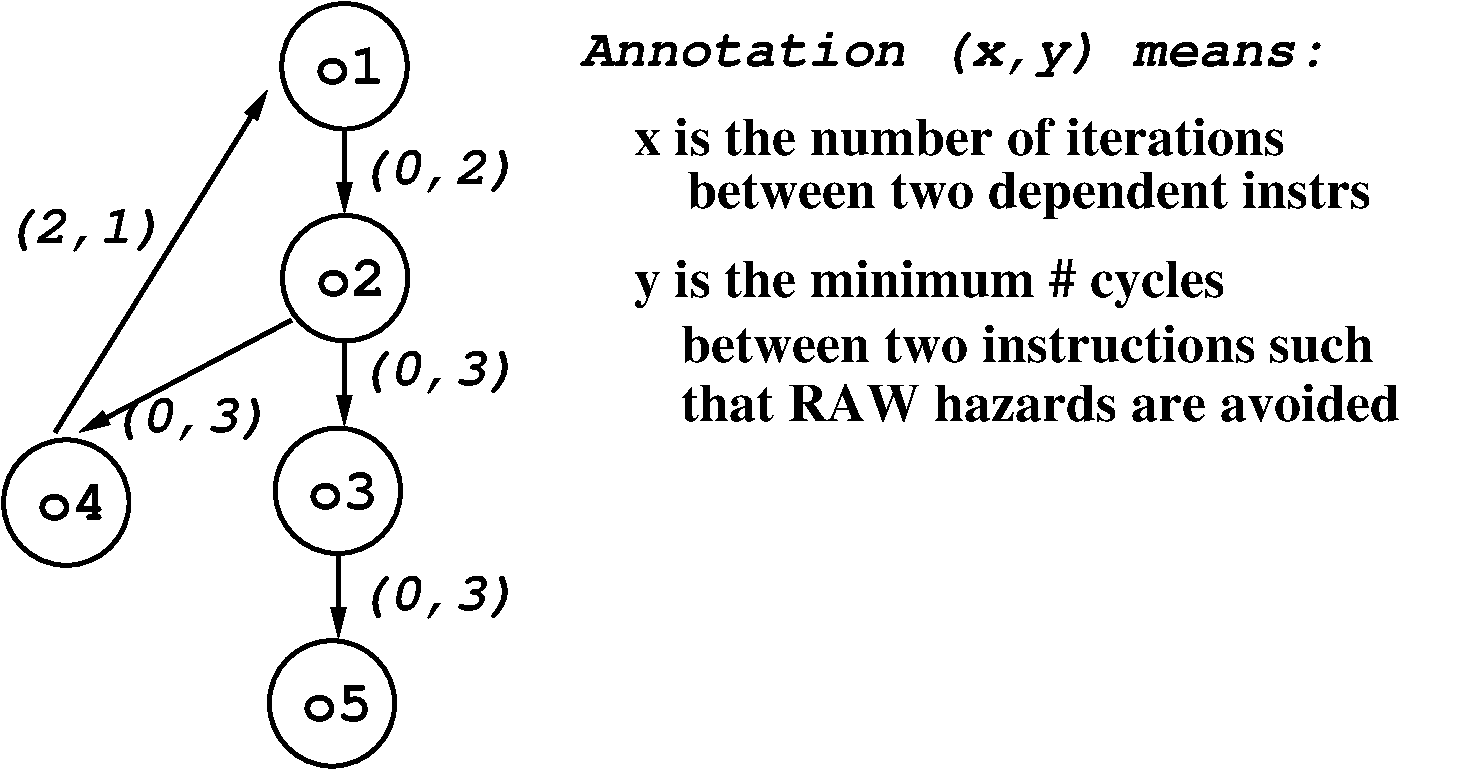
\includegraphics[width=27ex]{Figures/SftPipeDepGraph}
%\end{columns}
%\end{block}
%
%\bigskip
%
%\begin{scriptsize}
%\begin{itemize}
%    \item Loop-Carried Dependencies cause cycles in the graph \& limit the rate 
%            at which loop iterations can be scheduled:
%            \begin{itemize}
%           \begin{scriptsize}
%            \item graph-cycle straddles two iterations \& 
%            \item minimum \# of clocks to avoid RAW hazards is 6 $\Rightarrow$
%            \item Unsafe to schedule (original) loop iters faster than
%                    one every 6/2=3 cycles
%            \end{scriptsize}
%            \end{itemize}
%    \item Initiation Interval = 3 reaches a stable loop schedule,
%            that resolves all latencies; Otherwise increase it and try again!
%\end  {itemize}
%\end{scriptsize}
%\end{frame}
%
%\begin{frame}[fragile,t]
%    \frametitle{Software-Pipelining Schedule for Dependent Loop}
%
%\begin{tiny}
%\begin{tabular}{llllllll}
%\hline
%                 & O\_It1 & O\_It2 & O\_It3 & O\_It4  \\\hline
%\emp{P\_It1}     & o1     &        &        &         \\
%\emp{P\_It2}     & -      &        &        &         \\
%\emp{P\_It3}     & o2     &        &        &         \\
%\emp{P\_It4}     & -      & o1     &        &         \\
%\emp{P\_It5}     & -      & -      &        &         \\
%\emp{P\_It6}     & o3, o4 & o2     &        &         \\
%\emph{P\_It7}     & -      & -      & o1     &         \\
%\emph{P\_It8}     & -      & -      & -      &         \\
%\emph{P\_It9}     & o5     & o3, o4 & o2     &         \\
%\emp{P\_It10}    &        & -      & -      & o1      \\
%\emp{P\_It11}    &        & -      & -      & -       \\
%\emp{P\_It12}    &        & o5     & o3, o4 & o2      \\
%\emp{P\_It13}    &        &        & -      & -       \\
%\emp{P\_It14}    &        &        & -      & -       \\
%\emp{P\_It15}    &        &        & o5     & o3, o4  \\
%\end{tabular}
%\end{tiny}
%
%\smallskip
%
%\begin{scriptsize}
%\begin{itemize}
%    \item \emp{P\_It1-6 are the prolog}, \emph{P\_It7-9 are the loop body}, 
%          \emp{P\_It10-15 form the epilog.}
%        
%    \item Registers {\tt F3} and {\tt F4} are replaced with rotating registers
%            to solve WARs. 
%    \item {\tt F0} NOT replaced because is written \& consumed in
%            the same (pipelined) iteration.
%    \item The 3 VLIW instructions forming the pipelined-loop body are shown below:
%\end  {itemize}
%\end{scriptsize}
%
%\smallskip
%
%\begin{tiny}
%\begin{tabular}{llllll}
%\hline
%Clock   & MemOp1         & MemOp2         & FOp1            & FOp2             & Int/Branch \\\hline
%1       & NOOP           & L.S F0, 0(R2)  & NOOP            & NOOP             & DBNE R2,R4,Loop \\
%2       & NOOP           & NOOP           & NOOP            & NOOP             & ADDI R2,R2,\#8  \\
%3       & S.S RR2, 0(R2) & S.S RR0,-16(R3)& ADD.D RR3,F0,F1 & ADD.D RR1,RR2,F1 & ADDI R3,R3,\#8 \\\hline
%\end{tabular}
%\end{tiny}
%
%\end{frame}
%


\subsection{Trace Scheduling}

\begin{frame}[fragile,t]
    \frametitle{Non-Cyclic, Trace Scheduling}

Effective when a branch is highly predictable statically (profiling).

\begin{block}{Structure{\tt~~~}Original Code{\tt~~~~~}Trace Scheduled{\tt~~~~~~}Optim Code}\vspace{-1ex}
\begin{columns}
\column{0.18\textwidth}
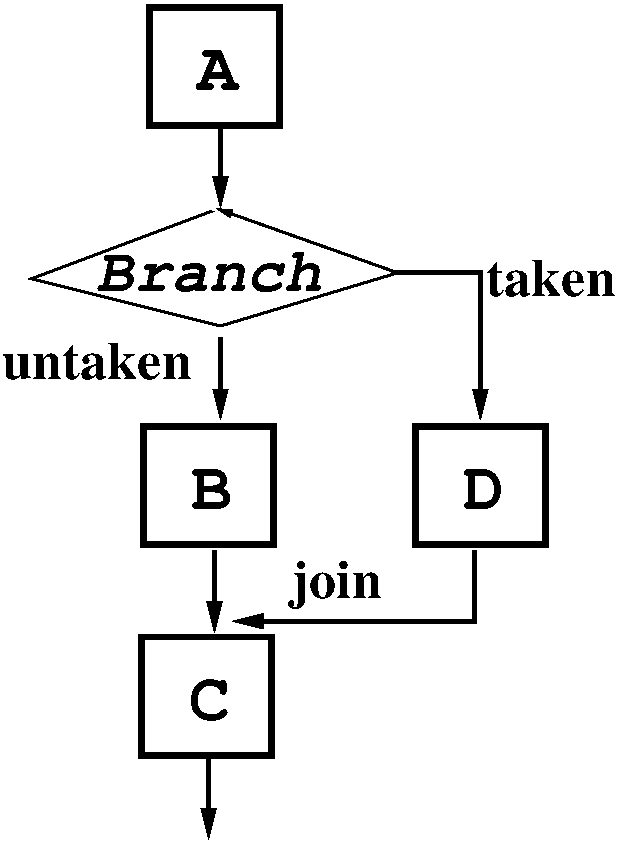
\includegraphics[width=13ex]{Figures/TraceSchedCFG}
\column{0.22\textwidth}
\begin{colorcode}[fontsize=\tiny]
      LW   R4, 0(R1)
      ADDI R6,R4,1
/* End Block A */
      BEQ  R5,R4,LAB
      LW   R6, 0(R2)
/* End Block B */
LAB:
/* End Empty Block D */
      SW   R6, 0(R2) 
/* End Block C */
\end{colorcode}
\column{0.25\textwidth}
\begin{colorcode}[fontsize=\tiny]
      LW   R4, 0(R1)
      ADDI R6,R4,1
      \emph{LW   R6, 0(R2)}
/* End Block A;B */
      BEQ  R5,R4,\emp{LABCC}
/*CompensationCode if taken*/
LAB:  
/* End Empty Block D */
      SW   R6, 0(R2) 
/* End Block C */
...
\emp{LABCC:}ADDI R6, R4, 1
      J    LAB
/*EndCompensationCode*/
\end{colorcode}
\column{0.23\textwidth}
\begin{colorcode}[fontsize=\tiny]
      \emph{LW   R4, 0(R1)}
      \emph{LW   R6, 0(R2)}
/* End Block A;B */
      BEQ  R5,R4,\emp{LABCC}
LAB:  SW   R6, 0(R2) 
/* End Block C */
...
\emp{LABCC:}  ADDI R6, R4, 1
        J    LAB
/*EndCompensationCode*/
\end{colorcode}
\end{columns}
\end{block}

\bigskip\pause

\begin{scriptsize}
\begin{itemize}
    \item Assume {\tt A$\rightarrow$B$\rightarrow$C} is the common path,
    \item Basic Blocks {\tt A} and {\tt B} are speculatively merged; 
    \item branch target is modified to jump to compensation code, from where
    \item it jumps back to the beginning of {\tt D}.
    \item Process can be repeated aggressively for branches in {\tt B}.
    \item Optimized Code: the two \emph{{\tt L.D}} can be scheduled in the same VLIW instruction.
\end  {itemize}
\end{scriptsize}
\end{frame}


\subsection{Predicated Instructions}

\begin{frame}[fragile,t]
    \frametitle{Predicated Instructions, e.g., IA-64}

Effective when branches:
\begin{itemize}
    \item are unbiased (50-50) or hard to predict statically, AND
    \item guard small basic blocks
\end  {itemize}

\begin{colorcode}[fontsize=\scriptsize]
    CLWZ  R1, 0(R2), R3   /* Load Mem[0(R2)] in R1 if R3 is     0 */
    CLWNZ R1, 0(R2), R3   /* Load Mem[0(R2)] in R1 if R3 is NOT 0 */
\end{colorcode}


\begin{block}{Original Code{\tt~~~~~~~~}Predicated{\tt~~~~~~~~~}Predicated Optim}\vspace{-1ex}
\begin{columns}
\column{0.33\textwidth}
\begin{colorcode}[fontsize=\tiny]
     LW   R4, 0(R1)
     ADDI R6, R4, #1
     \emp{BEQ  R5, R4, LAB}
     \emp{LW   R6, 0(R2)}
LAB: SW   R6, 0(R1)
\end{colorcode}
\column{0.31\textwidth}
\begin{colorcode}[fontsize=\tiny]
LW    R4, 0(R1)
ADDI  R6, R4, #1
\emph{SUB   R3, R5, R4}
\emph{CLWNZ R6, 0(R2), R3}
SW    R6, 0(R1)
\end{colorcode}
\column{0.31\textwidth}
\begin{colorcode}[fontsize=\tiny]
LW     R4, 0(R1)
SUB    R3, R5, R4
\emph{CADDIZ R6, R4, #1, R3}
\emph{CLWNZ  R6, 0(R2), R3}
SW     R6, 0(R1)
\end{colorcode}
\end{columns}
\end{block}

\bigskip

\begin{scriptsize}
\begin{itemize}
    \item \emp{{\tt BEQ} and {\tt LW}} translated as a \emph{predicated load, i.e., {\tt SUB} and {\tt CLWNZ}}.\pause
    \item Since {\tt R6} is overwritten when the conditional load holds, {\tt ADDI}
            is translated to its predicated form \emph{CADDIZ} which holds
            exactly when {\tt CLWNZ} does not.
    \item Now \emph{{\tt CLWNZ} and \emph{CADDIZ}} can be scheduled in the same VLIW instruction.
    \item Predicated instructions are not allowed to change the architectural state or to raise
            an exception unless their condition holds. 
    \item Predicated instructions transform control dependencies, which are a barrier
            to code motion, into data dependencies on registers, which are easier to handle.
\end  {itemize}
\end{scriptsize}
\end{frame}


\subsection{Speculative Memory Disambiguation}

\begin{frame}[fragile,t]
    \frametitle{Speculative Memory Disambiguation}

\emp{Problem:} A {\em load} cannot be moved across a {\em store} if it cannot be 
established statically that the two memory addresses are different.

\begin{block}{Original Code{\tt~~~~~~~~}Incorrect Code{\tt~~~~~~~~}Correct Code}\vspace{-1ex}
\begin{columns}
\column{0.31\textwidth}
\begin{colorcode}[fontsize=\scriptsize]
  I1
  SW  R1, 0(R3)
  I2
  LW  R4, 0(R2)
  ADD R5, R4, R4
\end{colorcode}
\column{0.31\textwidth}
\begin{colorcode}[fontsize=\scriptsize]
LW  R4, 0(R2)
ADD R5, R4, R4
I1
SW  R1, 0(R3)
I2
\end{colorcode}
\column{0.31\textwidth}
\begin{colorcode}[fontsize=\scriptsize]
\emph{LW.a R4, 0(R2)}
ADD  R5, R4, R4
I1
SW  R1, 0(R3)
I2
\emp{CHECK.a 0(R2), repair}
\end{colorcode}
\end{columns}
\end{block}

\bigskip

\begin{scriptsize}
\begin{itemize}
    \item The hoisted {\em load} is marked speculative via instruction \emph{{\tt LW.a}}, and
    \item a \emp{guardian} is inserted at the position from where it was moved.\pause\smallskip
 
    \item \emph{{\tt LW.a}} records its address in a small, fully associative table;
    \item Every store looks up and removes its address from this table;
    \item If the \emp{guardian} instruction \emp{CHECK.a} does not find the address in
            the table then a violation has occurred and a repair handle is launched. 
          In our case the latter re-executes the speculatively-hoisted instructions,
            i.e., {\tt LW} and {\tt ADD}.  
    \item \alert{Note that a {\em store} cannot be moved across a {\em load} because
            this miss-speculation cannot be easily repaired (memory is written). 
          Rather move the {\em store} downwards.}
\end  {itemize}
\end{scriptsize}
\end{frame}

\subsection{VLIW Handling of Exceptions}

\begin{frame}[fragile,t]
    \frametitle{VLIW Handling of Exceptions}

Cache misses freeze the pipeline $\Rightarrow$ compiler schedule is preserved.
\bigskip

Exceptions from cyclic scheduling NOT a problem because all instrs of the transformed
program are also executed in the original program.
\bigskip

Exception from \emp{non-cyclic scheduling are problematic} because speculatively
executed instructions may trigger exceptions that would not arise in the original code,
e.g., array out of bounds.
  
\begin{scriptsize}
\begin{itemize}
    \item User-invisible exceptions are harmless and can always be taken, 
            e.g., page faults caused by speculative memory disambiguation.\smallskip
    \item Unwanted User-Visible Exceptions, e.g., termination due to index out of 
            bounds caused by a speculative load, 
            must be repressed if speculation does not hold.
\end  {itemize}
\end{scriptsize}

\bigskip

A common solution is {\bf deferred exceptions}: whenever a speculative 
instruction triggers a user-visible exception, the destination register
is poisoned (poisoned bit set \& exception report).  

\end{frame}


\begin{frame}[fragile,t]
    \frametitle{VLIW Handling of Exceptions (Cont.)}

Deferred Exceptions via Poisoning:
\begin{scriptsize}
\begin{itemize}
    \item When another speculative instruction reads a poisoned value, poison
            is propagated to its destination register as well, without raising 
            exception.\smallskip
    \item When an instruction with no exception writes a poisoned register,
            the poison bit is reset $\Rightarrow$ the poisoned value
            was useless.\smallskip
    \item \emp{Exception is taken when a non-speculative instr 
                uses a poisoned value (as operand)}.
\end  {itemize}
\end{scriptsize}


\smallskip

\begin{block}{Orignal{\tt~~~~~~}Trace Scheduled{\tt~~~~~~~~}Deferred Exception}\vspace{-1ex}
\begin{columns}
\column{0.31\textwidth}
\begin{colorcode}[fontsize=\tiny]
      LW   R4, 0(R1)
      ADDI R6,R4,1
      BEQ  R5,R4,LAB
      LW   R6, 0(R2)
LAB:  SW   R6, 0(R2) 
\end{colorcode}
\column{0.31\textwidth}
\begin{colorcode}[fontsize=\tiny]
      LW   R4, 0(R1)
      ADDI R6,R4,1
      \alert{LW   R6, 0(R2)}
      BEQ  R5,R4,LABCC
LAB:  SW   R6, 0(R2) 
...
LABCC:ADDI R6, R4, 1
      J    LAB
/*Compensation Code*/
\end{colorcode}
\column{0.31\textwidth}
\begin{colorcode}[fontsize=\tiny]
      LW   R4, 0(R1)
      ADDI R6,R4,1
      \emp{sLW  R6, 0(R2)}
      BEQ  R5,R4,LABCC
LAB:  \emph{SW   R6, 0(R2)} 
...
\emph{LABCC:ADDI R6, R4, 1}
      J    LAB
/*Compensation Code*/
\end{colorcode}
\end{columns}
\end{block}


\begin{scriptsize}
\begin{itemize}
    \item When a user-visible exception occurs on \emp{sLW} $\Rightarrow$ {\tt R6} is poisoned:\smallskip
    \item If branch is taken\pause poison goes away because {\tt R6} is re-written 
            ({\tt LABCC: ADDI}). \emph{This is Correct Behavior}: branch
            was miss-speculated \& the load should not have occurred. 
    \item If branch is not taken, then the exception is raised by non-speculative
            {\tt SW} which uses {\tt R6}. \emph{Again, Correct Behavior}:
            the speculation was correct and resulted in exception.
\end  {itemize}
\end{scriptsize}

\end{frame}


%%%%%%%%%%%%%%%%%%%%%%%%%%%%%%%%%%%%%%%%%%%%%%%%%%%%%
%%%%%%%%%%%%%%%%%%%%%%%%%%%%%%%%%%%%%%%%%%%%%%%%%%%%%
%%%%%%%%%%%%%%%%%%%%%%%%%%%%%%%%%%%%%%%%%%%%%%%%%%%%%
\section{Basic Blocks, CFG, Loops, Reducible CFG, Simple Optims}

\begin{frame}[fragile]
	\tableofcontents[currentsection]
\end{frame}


\begin{frame}[fragile,t]
    \frametitle{Basic Blocks \& Control Flow Graph}

We use Three Address Code ({\sc tac}) rather than MIPS:\smallskip\pause
\begin{itemize}
\item instruction has at most 2 operands \& one result, e.g., {\tt s := s+i}\smallskip
\item Jump labels, {\tt goto}, conditional jump ({\tt if}), e.g., {\tt if i=0 goto L2}\smallskip
\item Memory load/store, function call/return (not used here).\smallskip
\end{itemize}

\bigskip

\begin{block}{Three Address Code Example}
\begin{colorcode}[fontsize=\scriptsize]
    i := 20
    s := 0
L1: if i=0 \emp{goto L2}
    s := s + i
    i := i - 1
    \emp{goto L1}
L2: ...
\end{colorcode} 
\end{block}

\bigskip

Interm-lang optimizations, e.g., \textsc{TAC}, portable to various backends, \smallskip
$\ldots$ but \emp{Can we rebuild the control flow structure from {\sc tac}?}

\end{frame}

\subsection{Basic Blocks Constructions and The Control-Flow Graph}

\begin{frame}[fragile,t]
    \frametitle{Basic Blocks (BB)}

Basic Block: intuitively the maximal sequence of (consecutive) {\sc tac} 
                instructions in which flow can enter/exit only via 
                the first/last instr.

\bigskip

\begin{block}{Code Example $\mbox{~~~~~~~~~~~~~~~~~}$ Incorrect Basic Block}
\begin{columns}
\column{0.33\textwidth}
\begin{colorcode}[fontsize=\scriptsize]
    i := 20
    s := 0
L1: if i=0 \emp{goto L2}
    s := s + i
    i := i - 1
    \emp{goto L1}
L2: ...
\end{colorcode}
\column{0.55\textwidth}
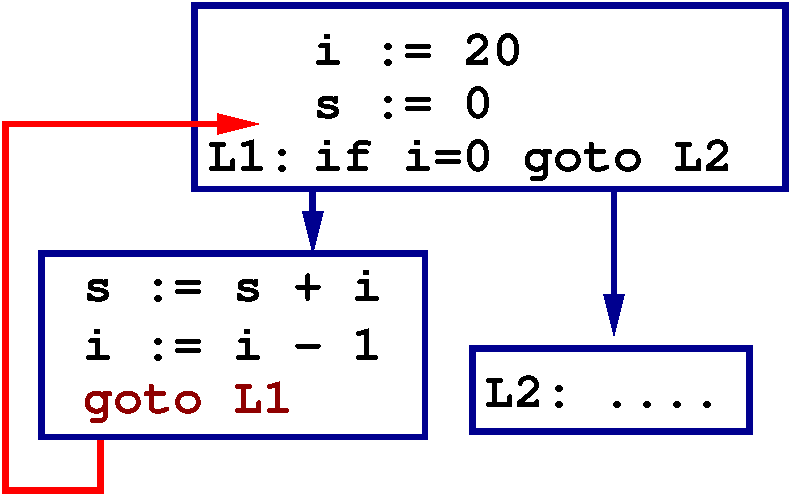
\includegraphics[width=20ex]{Figures/CFGwrong}
\end{columns} 
\end{block}

\end{frame}


\begin{frame}[fragile,t]
    \frametitle{Identifying Basic Blocks (BB)}

\begin{itemize}
\item Statements that \blue{start a basic block (BB)}:
    \begin{itemize}
        \item first statement of any function

        \item any labeled statement that is the target of a branch

        \item any statement following a branch (conditional or unconditional)\smallskip
    \end{itemize}

\item \blue{for each statement starting a BB}, the BB consists of all stmts up
            to, but excluding, the start of a BB or the end of the program!
\end{itemize}
\end{frame}


\begin{frame}[fragile,t]
    \frametitle{Identifying Basic Blocks (BB)}

\begin{itemize}
\item Statements that \blue{start a basic block (BB)}:
    \begin{itemize}
        \item first statement of any function

        \item any labeled statement that is the target of a branch

        \item any statement following a branch (conditional or unconditional)\smallskip
    \end{itemize}

\item \blue{for each statement starting a BB}, the BB consists of all stmts up
            to, but excluding, the start of a BB or the end of the program!
\end{itemize}

\begin{block}{Code Example $\mbox{~~~~~~~~~~~~~~~~~}$ Basic Blocks}
\begin{columns}
\column{0.33\textwidth}
\begin{colorcode}[fontsize=\scriptsize]
    \blue{i := 20}
    s := 0
\blue{L1:} if i=0 \emp{goto L2}
    \blue{s := s + i}
    i := i - 1
    \emp{goto L1}
\blue{L2: ... }
\end{colorcode} 
\column{0.55\textwidth}
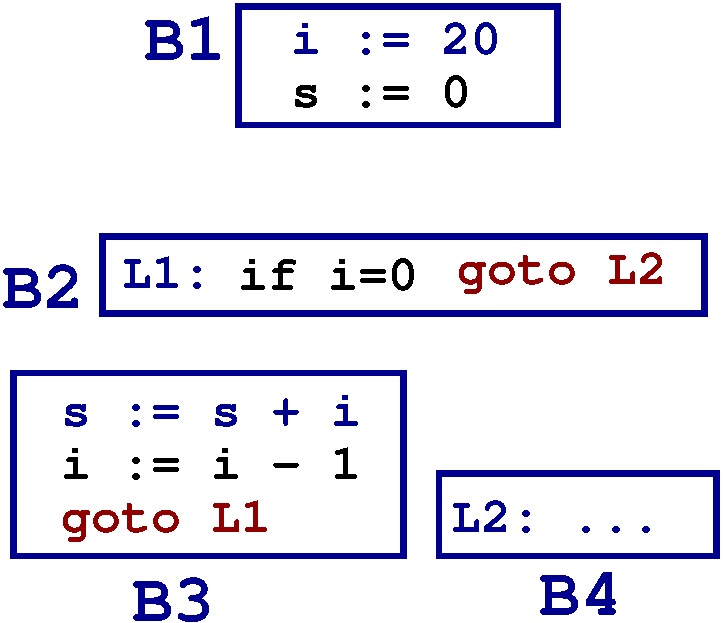
\includegraphics[width=20ex]{Figures/CFGbb}
\end{columns}
\end{block}

\end{frame}


\begin{frame}[fragile,t]
    \frametitle{Building The Control-Flow Graph}


Place an arrow from node $A$ to node $B$ if it is possible 
for control to ``flow'' from $A$ to $B$ (and remove gotos).

\bigskip

\begin{block}{Code Example and its Control-Flow Graph ({\sc CFG})}
\begin{columns}
\column{0.33\textwidth}
\begin{colorcode}[fontsize=\scriptsize]
    \blue{i := 20}
    s := 0
\blue{L1:} if i=0 \emp{goto L2}
    \blue{s := s + i}
    i := i - 1
    \emp{goto L1}
\blue{L2: ... }
\end{colorcode} 
\column{0.55\textwidth}
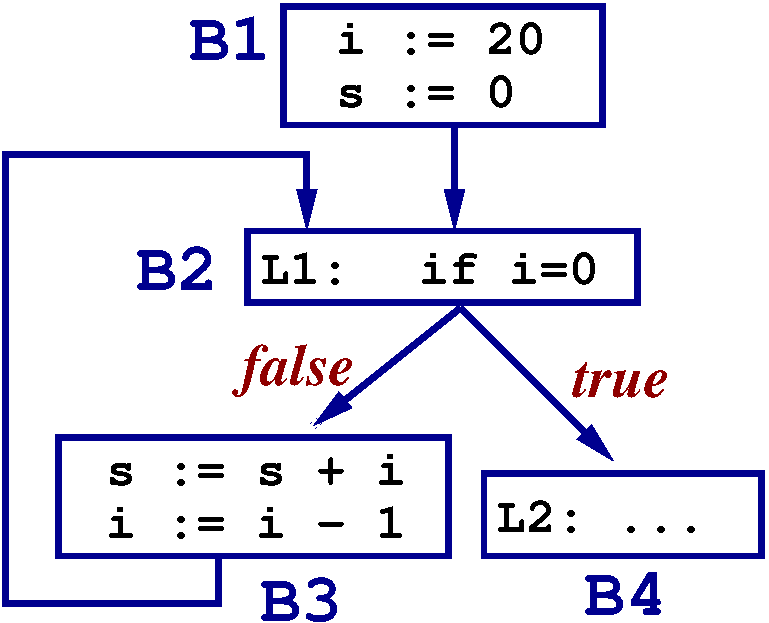
\includegraphics[width=20ex]{Figures/CFGeg}
\end{columns}
\end{block}

\end{frame}


\subsection{Identifying Loops}


\begin{frame}[fragile,t]
    \frametitle{Identifying Loops, Preliminaries}

{\bf Motivation}: loops is where most of the time is spent!

\pause
\bigskip

{\bf Definition}: A loop, $L$, is a subgraph of the \textsc{CFG} such that:

\begin{itemize}

\item all nodes of the loop are \emp{strongly connected}, i.e., the loop
        contains a path between any two loop nodes.

\item the loop has \green{an unique entry point}, named \emph{header}, such that

\item the only way to reach a loop node is through the entry point.

\end{itemize}

A loop that contains no other loop is called an {\em innermost loop}.

\pause
\bigskip

{\bf Dominator Definition}: a node $p$ \emp{dominates} node $q$ if all paths from
the start of the program to $q$ go through $p$.

\bigskip

{\bf Identifying} loops requires finding their ``\emp{back edges}'':

\begin{itemize}

\item edges in the program in which the destination node dominates
        the source node.

\item a loop must have \green{an unique header}, and \emp{one or more backedges}.

\item header dominates all blocks in the loop, otherwise not unique.

\end{itemize}

\end{frame}





\begin{frame}[fragile,t]
    \frametitle{Example of a Loop CFG}

\bigskip

\begin{block}{Example: Finding Basic Blocks and The Control-Flow Graph (CFG)}
\begin{columns}
\column{0.3\textwidth}
\begin{colorcode}[fontsize=\scriptsize]
    s := 0
    i := 0
    n := 10
\blue{L1:}
    t1 := a - b
    if t1 = 0 \emp{goto L2}
    t2 := i * 4
    s := s + t2
    \emp{goto L3}
\blue{L2:} s := s + i
\blue{L3:} i := i + 1
    t3 := n - i
    if t3 != 0 \emp{goto L1}
    t4 := a - b
    CALL PRINT(t4)
\end{colorcode} 
\column{0.6\textwidth}
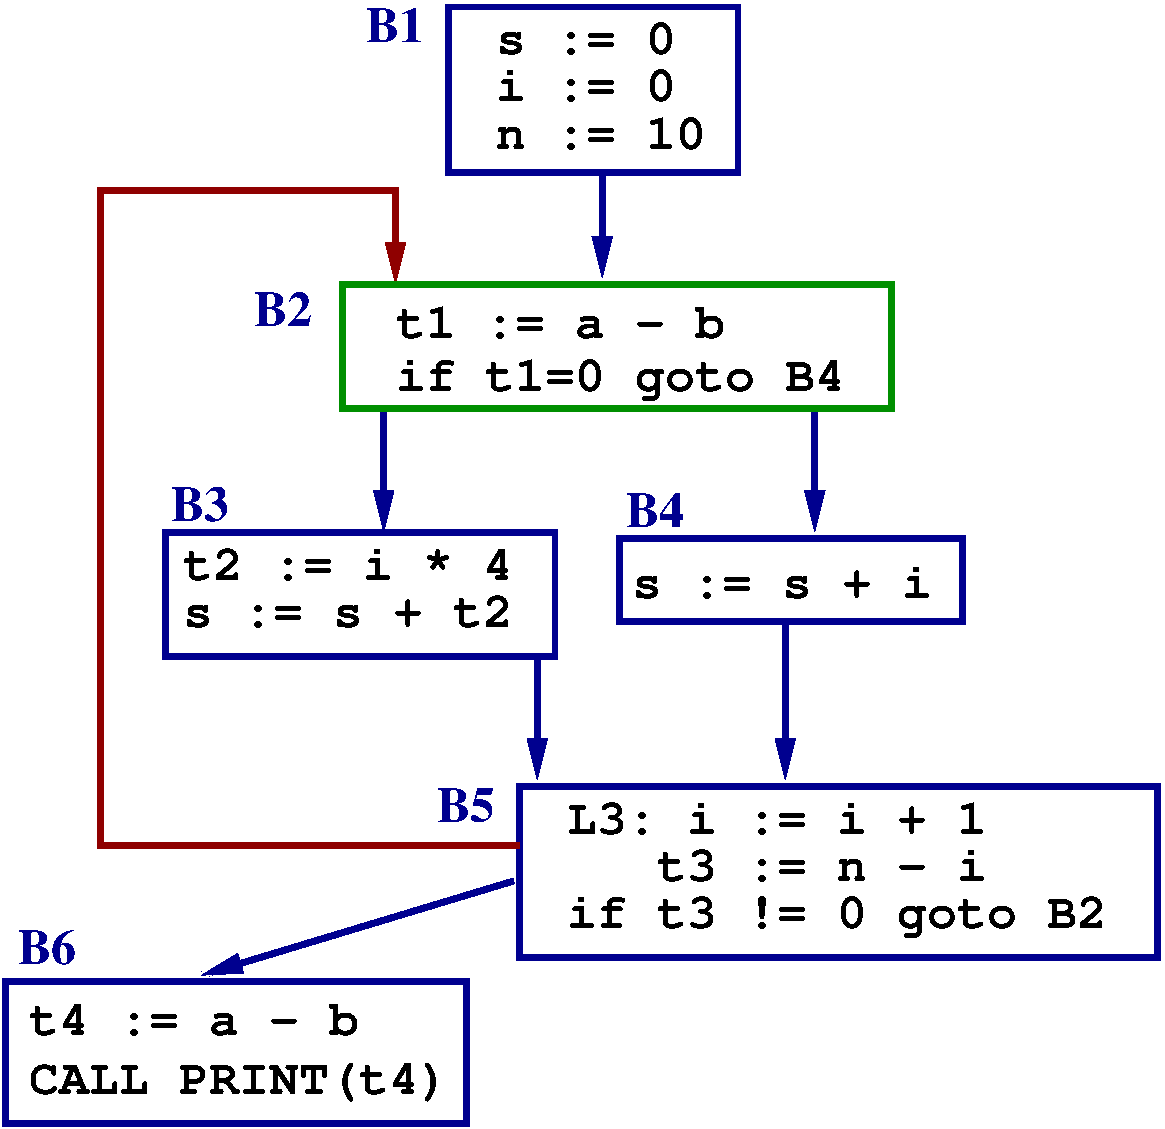
\includegraphics[width=33ex]{Figures/LoopEg}
\end{columns}
\end{block}

\end{frame}





\begin{frame}[fragile,t]
    \frametitle{Identifying Loops}

\begin{block}{Algorithm for Dominators. $D(n)$ is the set of dominators of block $n$.}
%\begin{colorcode}[fontsize=\scriptsize]
{\bf Input}: \textsc{CFG} with node set $N$, initial node $n_0$.
{\bf Output}: $D(n), \forall n \in N$\\
{\tt~~}\\
$D(n_0) := \{ n_0 \}$\\
for $n \in N - \{n_0\}$ do $D(n)$ := $N$\\
{\tt~~}\\
while changes to any $D(n)$ occur do\\
{\tt~~~~}for $n \in N - \{n_0\}$ do\\
{\tt~~~~~~~~}$D(n)$ := $\{n\} \cup \alert{(\cap_{p\in pred(n)} D(p))}$
%\end{colorcode} 
\end{block}

\pause
\bigskip

{\bf High-Level Algorithm}: With each \emp{backedge $n \rightarrow d$}
($d$ is the loop header), we associate a \green{natural loop} (of $n \rightarrow d$) 
consisting of node $d$ and all nodes that can reach $n$ without going through $d$.

\bigskip

{\bf Intuition}: since $d$ is the only entry to the loop, a path from any
block outside the loop must pass through $d$.

\end{frame}



\subsection{Control-Flow-Graph Reducibility}

\begin{frame}[fragile,t]
    \frametitle{Reducible Control-Flow Graphs ({\sc CFG})}

%(Assumes I have already introduce dominators, back-edges, loops).


{\bf A CFG is reducible} if it can be partitioned in forward and backward
edges, and the forward edges form a directed-acyclic graph.\smallskip

\begin{block}{{\tt~~~}Reducible CFG{\tt~~~~~~~~~~~~~~~~}Irreducible CFG}
\begin{columns}
\column{0.45\textwidth}
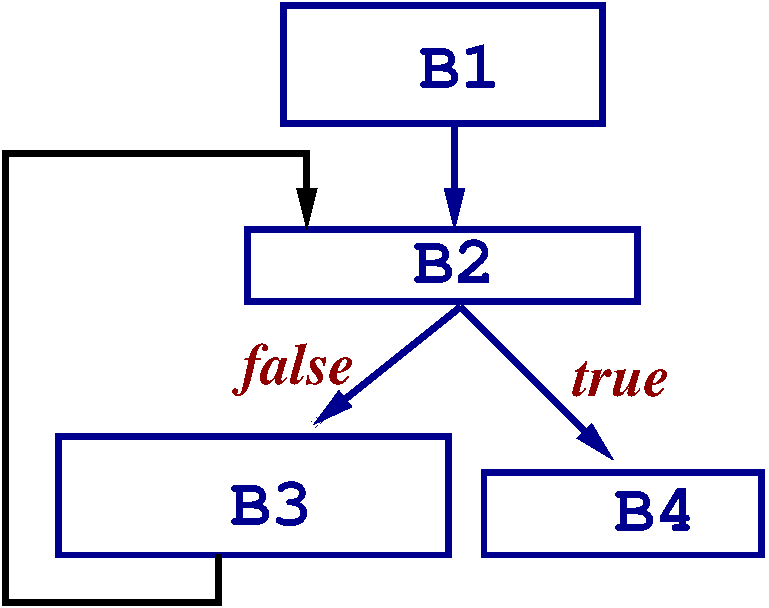
\includegraphics[width=20ex]{Figures/CFGred}
\column{0.45\textwidth}
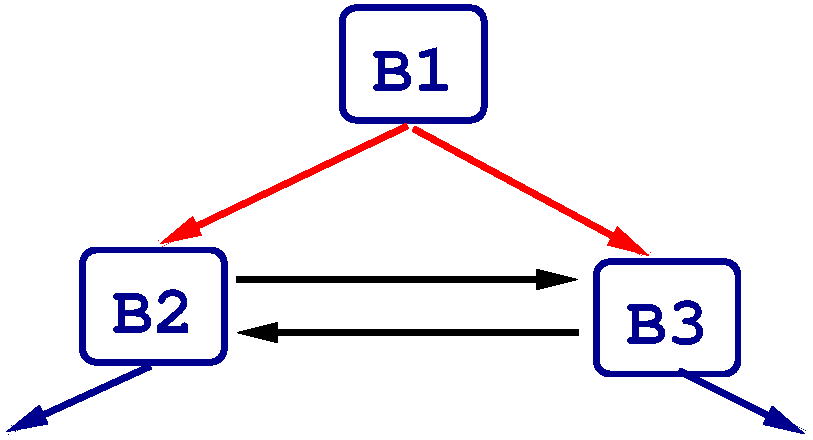
\includegraphics[width=20ex]{Figures/LoopUnstruct}
%\column{0.30\textwidth}
%\includegraphics[width=20ex]{Figures/NodeCloning}\\
%\alert{Exponential code explosion is possible.}
\end{columns}
\end{block}

\smallskip

Irreducible {\sc cfg}: due to unstructured GOTOs,\\e.g., jumps in the middle of a loop.

\smallskip

\emp{\em How to test {\sc cfg} reducibility?}

\end{frame}




\begin{frame}[fragile,t]
    \frametitle{Testing CFG Reducibility via T1-T2 Transformation}

{\bf Why Is Reducibility Important?} 1. A reducible {\sc cfg} can be written
only in terms of (while/do) loops, if statements and function calls.

\bigskip

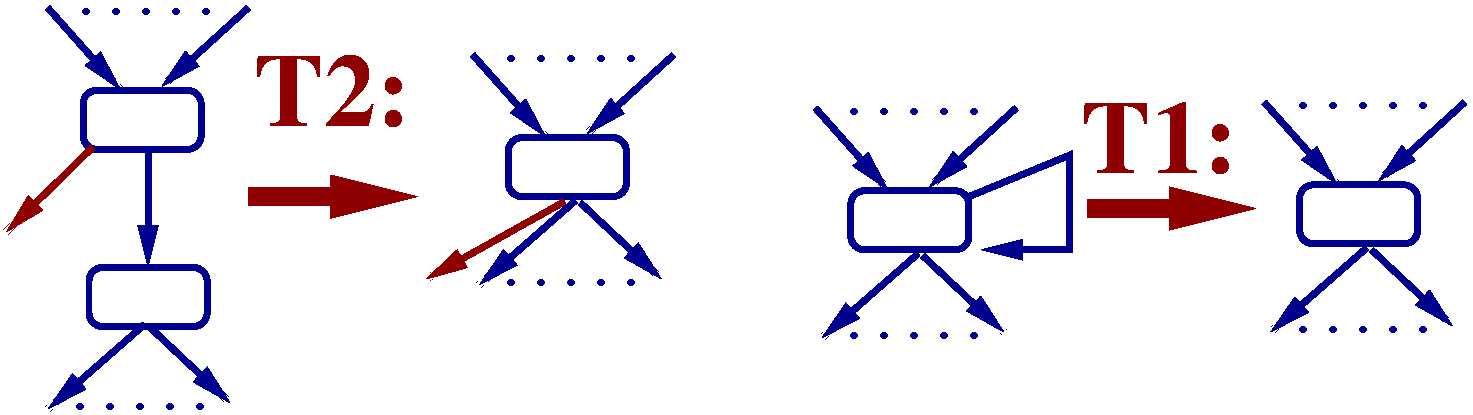
\includegraphics[width=44ex]{Figures/CFG_T12}

{\bf Reducible CFG} {\em iff} can be reduced to 1 node via T1/T2 applications.\smallskip

\begin{block}{{\tt~~~}Reducible CFG via T2}
\begin{columns}
\column{0.18\textwidth}
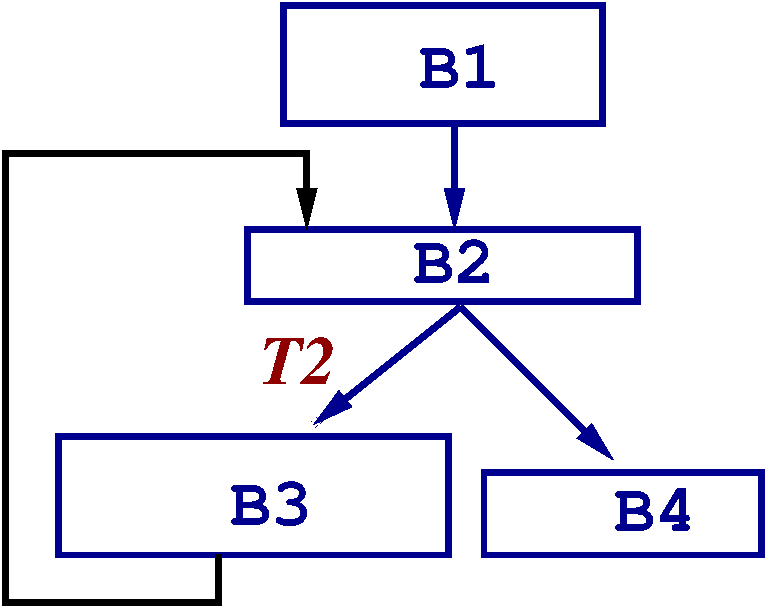
\includegraphics[width=15ex]{Figures/CFGred1}
\column{0.15\textwidth}
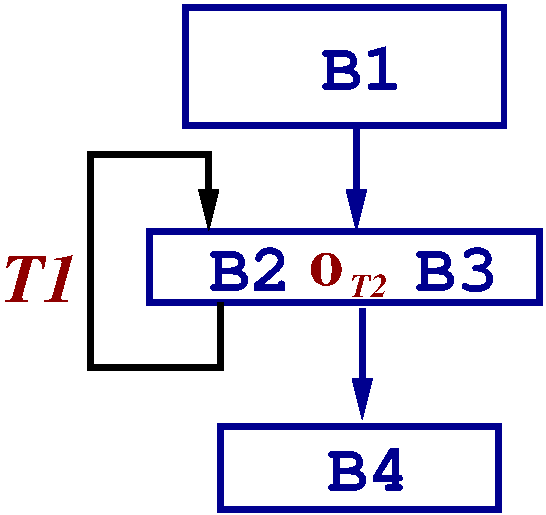
\includegraphics[width=11ex]{Figures/CFGred2}
\column{0.15\textwidth}
%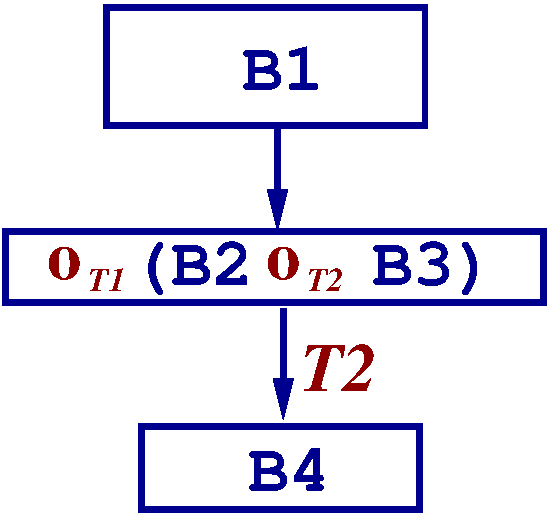
\includegraphics[width=11ex]{Figures/CFGred3}
\column{0.33\textwidth}
%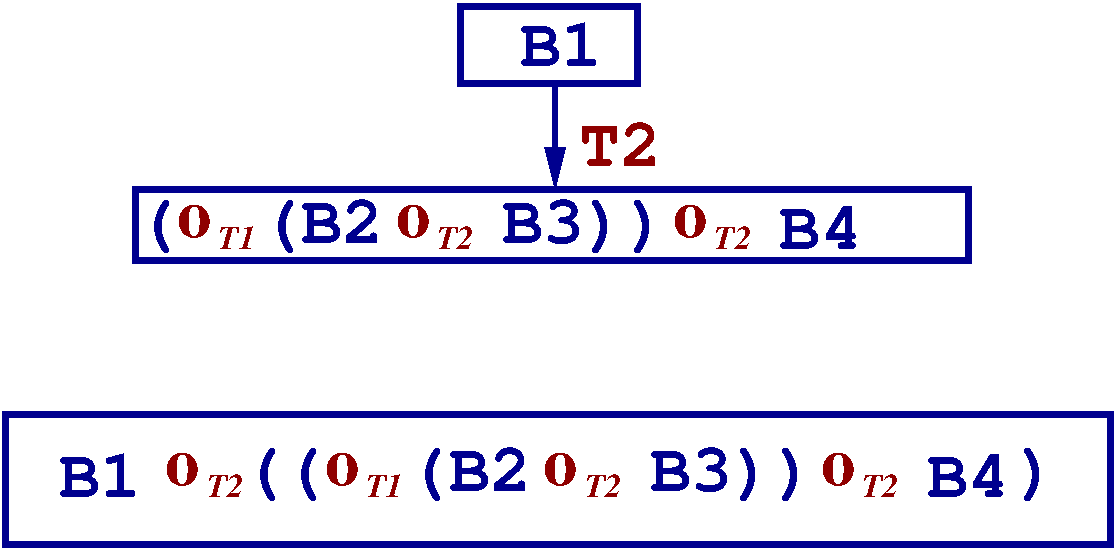
\includegraphics[width=22ex]{Figures/CFGred4}
\end{columns}
\end{block}

\end{frame}

\begin{frame}[fragile,t]
    \frametitle{Testing CFG Reducibility via T1-T2 Transformation}

{\bf Why Is Reducibility Important?} 1. A reducible {\sc cfg} can be written
only in terms of (while/do) loops, if statements and function calls.

\bigskip

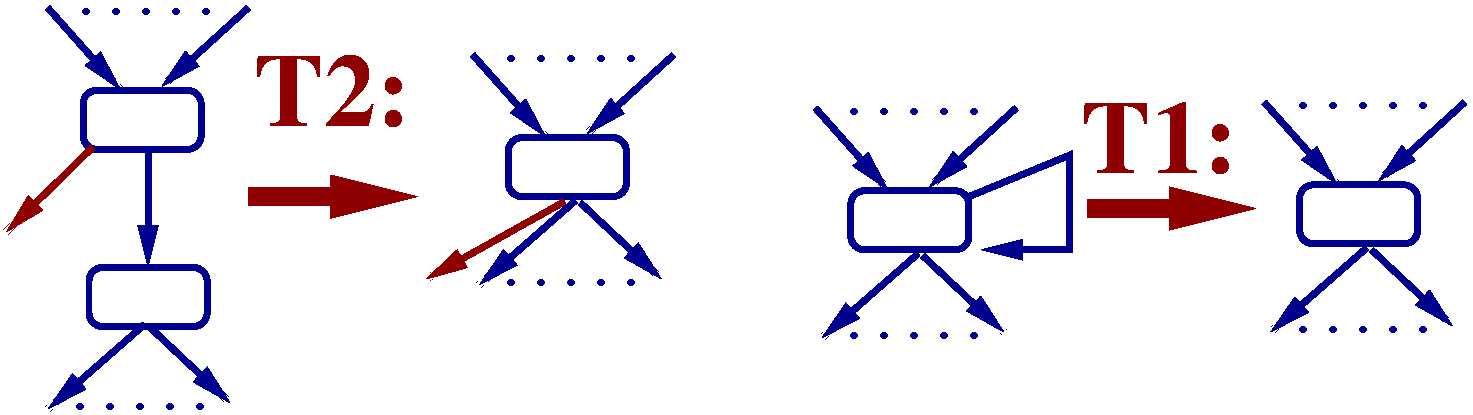
\includegraphics[width=44ex]{Figures/CFG_T12}

{\bf Reducible CFG} {\em iff} can be reduced to 1 node via T1/T2 applications.\smallskip

\begin{block}{{\tt~~~}Reducing CFG via T1}
\begin{columns}
\column{0.18\textwidth}
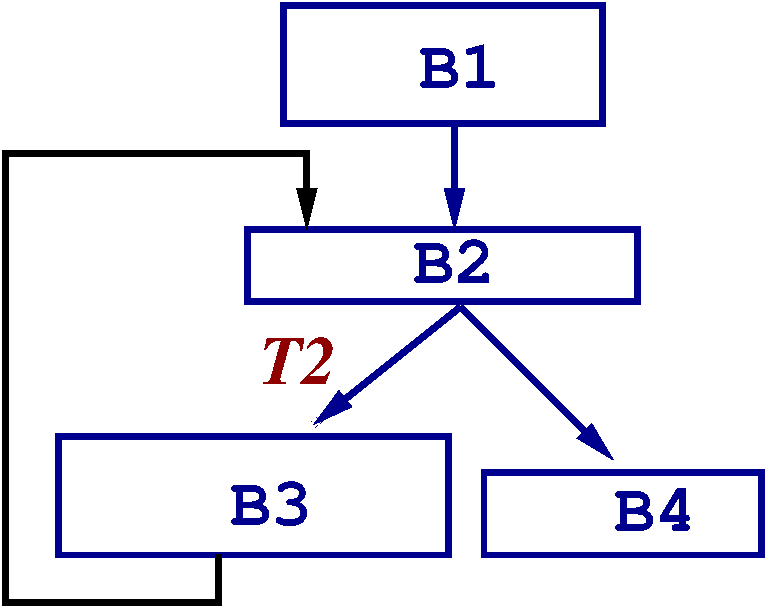
\includegraphics[width=15ex]{Figures/CFGred1}
\column{0.15\textwidth}
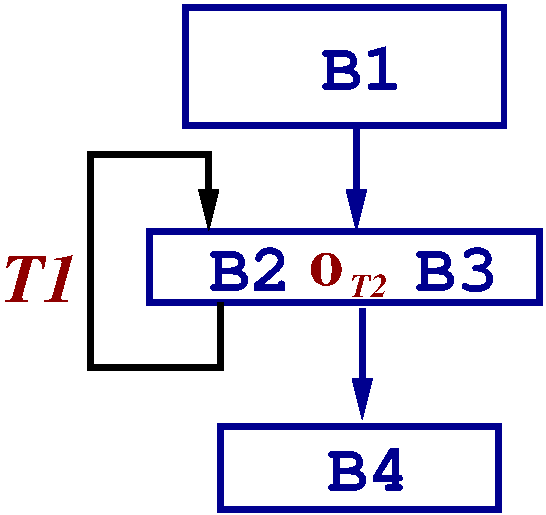
\includegraphics[width=11ex]{Figures/CFGred2}
\column{0.15\textwidth}
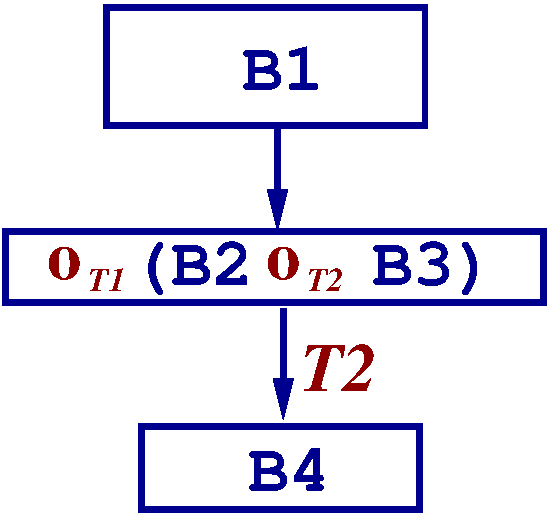
\includegraphics[width=11ex]{Figures/CFGred3}
\column{0.33\textwidth}
%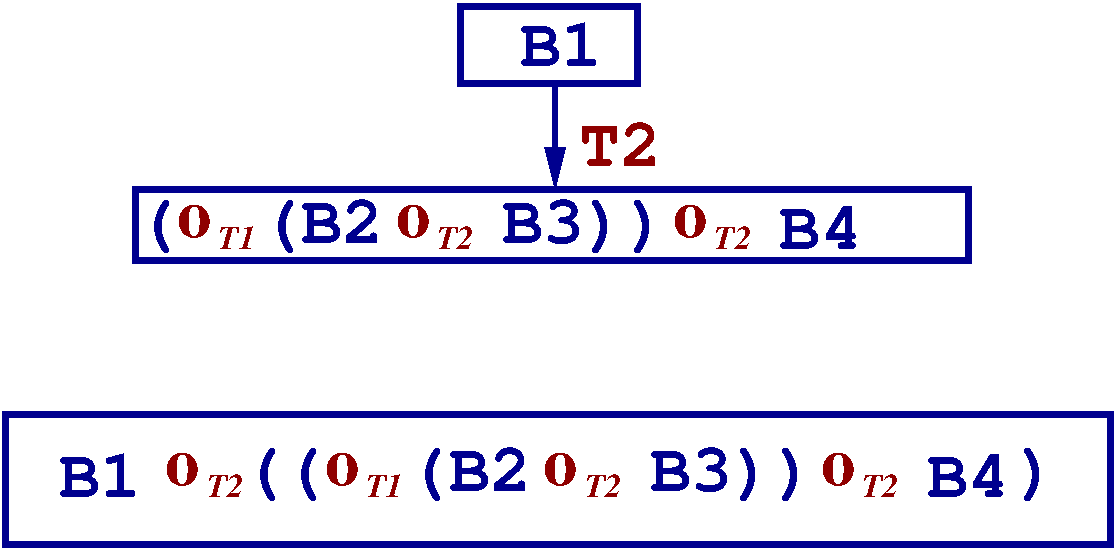
\includegraphics[width=22ex]{Figures/CFGred4}
\end{columns}
\end{block}

\end{frame}


\begin{frame}[fragile,t]
    \frametitle{Testing CFG Reducibility via T1-T2 Transformation}

{\bf Why Is Reducibility Important?} 2. If \textsc{AbSyn} guarantees 
reducible {\sc cfg} then data-flow rules associated with each 
\textsc{AbSyn} node; the result is composed in \emph{one program traversal}, 
rather than \emp{fix-point iter}. 

\bigskip

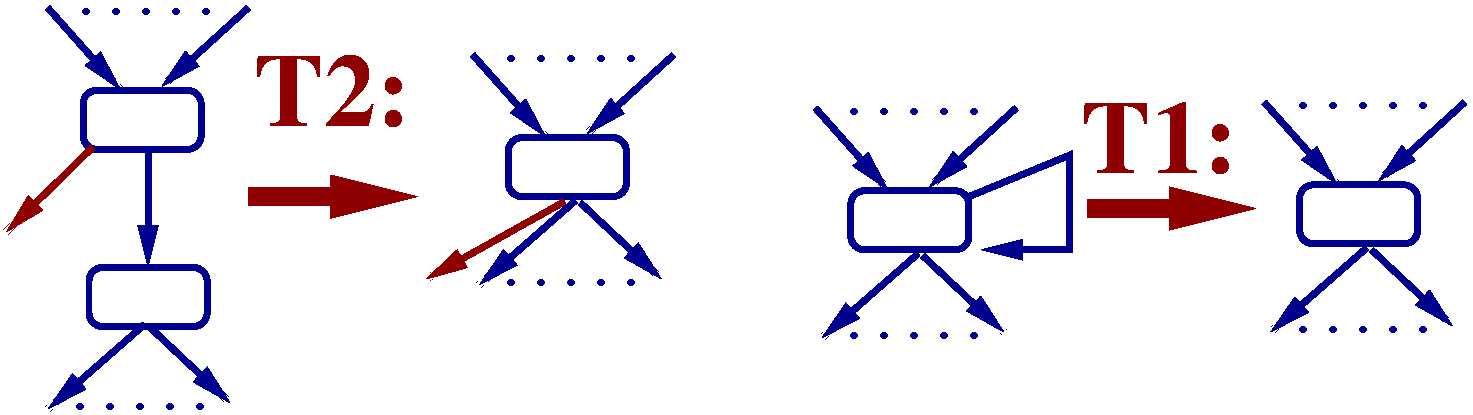
\includegraphics[width=44ex]{Figures/CFG_T12}

{\bf Reducible CFG} {\em iff} can be reduced to 1 node via T1/T2 applications.\smallskip


\begin{block}{{\tt~~~}Reducing CFG via T2}
\begin{columns}
\column{0.18\textwidth}
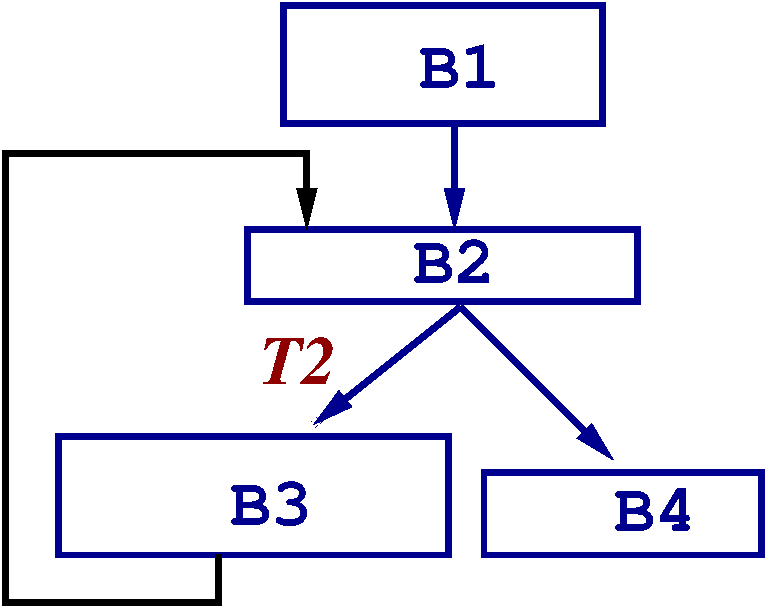
\includegraphics[width=15ex]{Figures/CFGred1}
\column{0.15\textwidth}
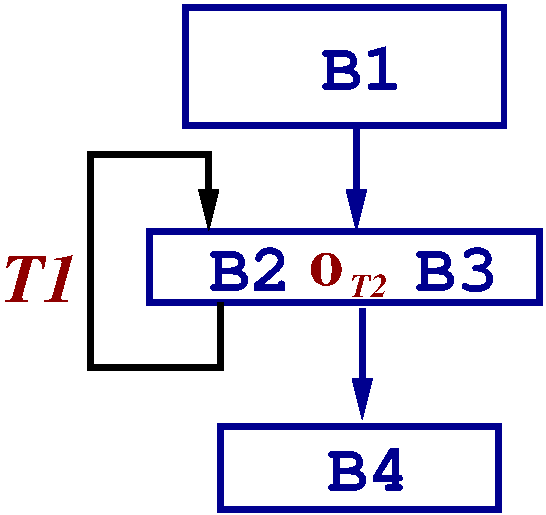
\includegraphics[width=11ex]{Figures/CFGred2}
\column{0.15\textwidth}
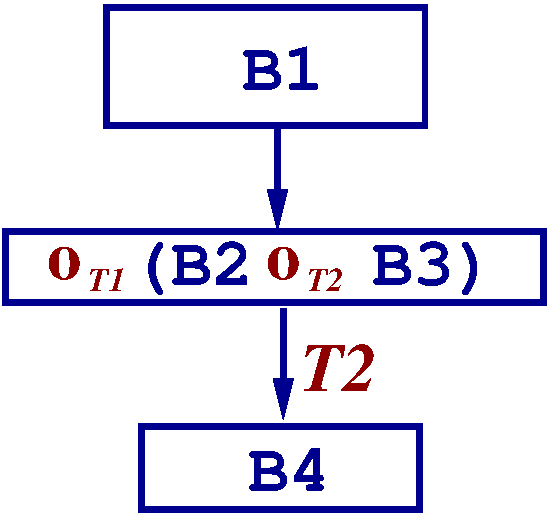
\includegraphics[width=11ex]{Figures/CFGred3}
\column{0.33\textwidth}
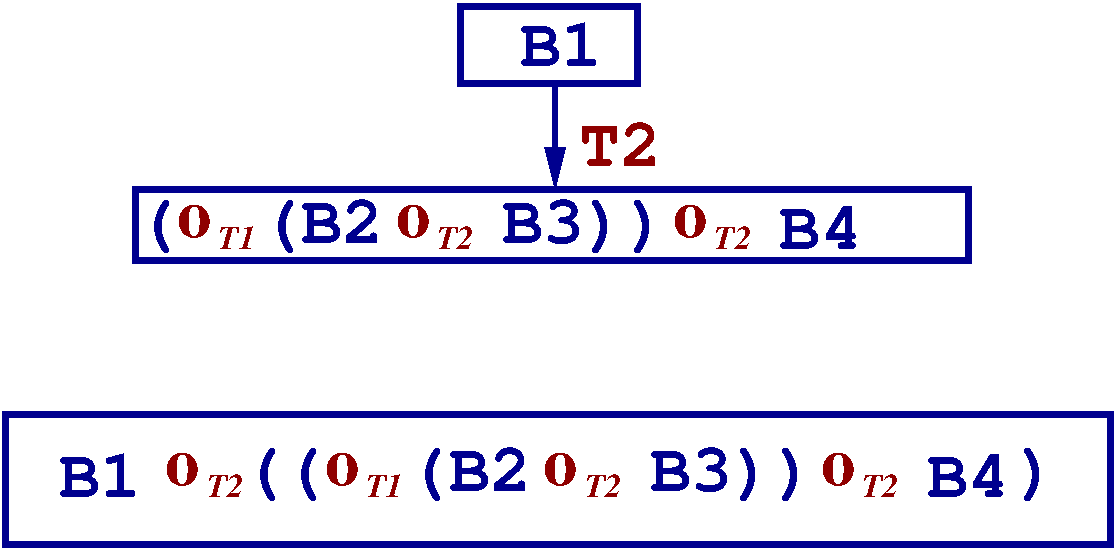
\includegraphics[width=22ex]{Figures/CFGred4}
\end{columns}
\end{block}

\end{frame}


\begin{frame}[fragile,t]
    \frametitle{Testing and Solving Ireducible CFG}

\bigskip

\begin{block}{Alg for Testing Reducibility{\tt~~~~~~~~~~}Node Splitting}
\begin{columns}
\column{0.41\textwidth}
In a copy of the \textsc{CFG}, apply\\
{\tt T1} and {\tt T2} to a fixpoint. If\\
the result is a single node\\
than the \textsc{CFG} is reducible.\\
%
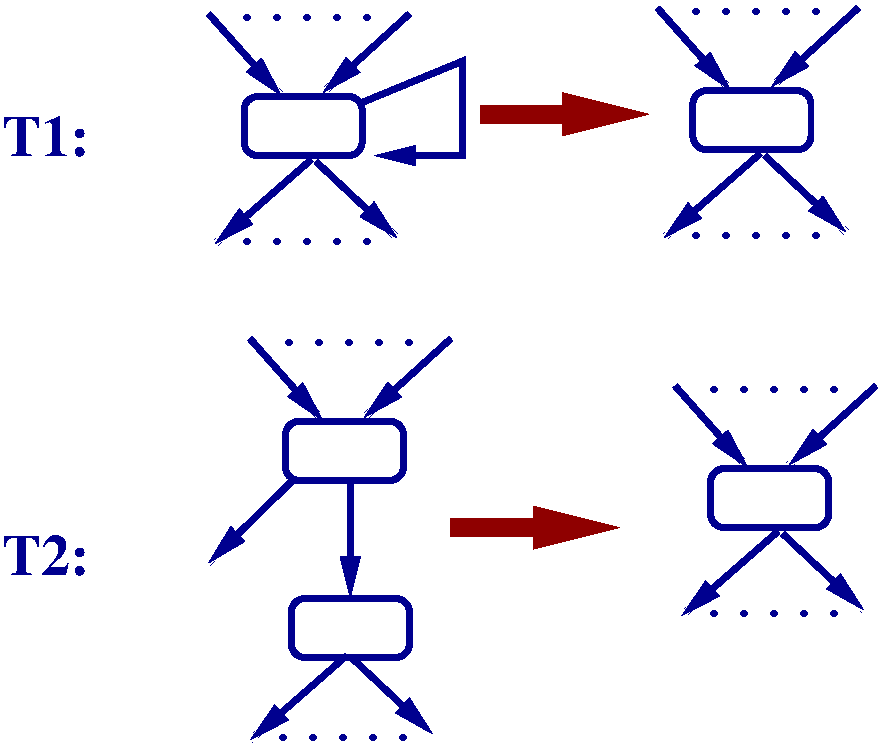
\includegraphics[width=17ex]{Figures/T12}
\column{0.55\textwidth}
Irreducible \textsc{CFG}s are difficult to\\
optimize. It is always possible to solve\\
irreducibility, but, in the worst case, at\\
the cost of an exponential-code explosion:\\
%
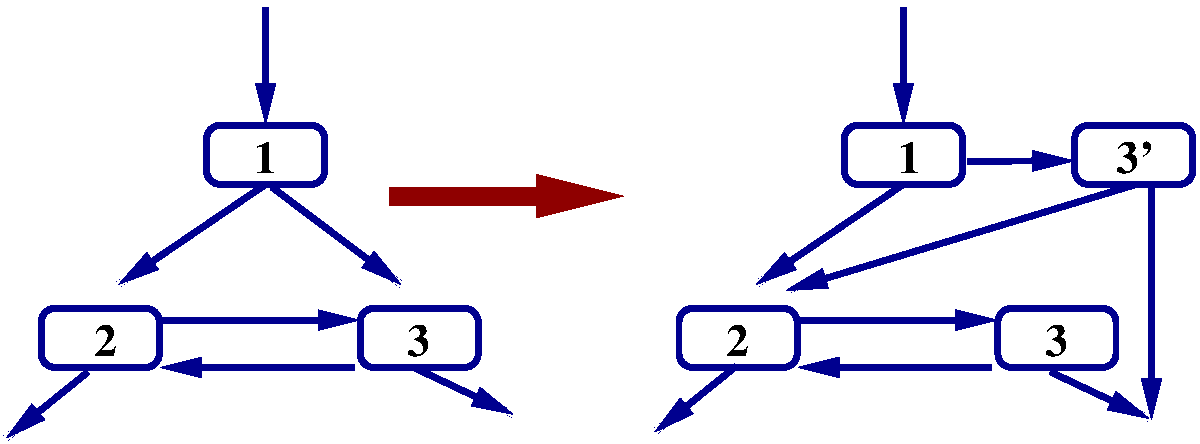
\includegraphics[width=34ex]{Figures/NodeSplit}
\end{columns}
\end{block}

{\bf Key property}: if a CFG is reducible then all cycles are (regular)
loops, and identifying the backedges is enough to find all loops.


\end{frame}


\begin{frame}[fragile,t]
    \frametitle{CFG Reducibility via T1-T2 Transformation}

{\bf Why Is Reducibility Important?} 2. If \textsc{AbSyn} guarantees 
reducible {\sc cfg} then equations associated with each \textsc{AbSyn} node;
the result is composed in \emph{one program traversal}, rather than \emp{fix-point iteration}. 

\bigskip

This allows optimizations to be implemented in the simpler, 
intuitive case-analysis style, e.g., live-function computation:

\smallskip

%\begin{block}{ Computing Live Functions }
%\begin{colorcode}[fontsize=\scriptsize]
%fun \emp{live_funs} (exp, ftab, livefs: string list) : string list =
%case exp of
%  If(e1, e2, e3) => foldl ( fn(e,lives)=>\emp{live_funs}(e, ftab, lives) ) 
%                          livefs [e1,e2,e3]
%| ... 
%\end{colorcode}
%\end{block}

\begin{block}{Pseudocode for computing the live functions (names)}
\begin{colorcode}[fontsize=\scriptsize]
fun live_funs ( exp, ftab, livefs : string list ) : string list =
  case exp of
    Plus (e1, e2, pos) =>
        \emph{live_funs(e2, ftab, live_funs(e1, livefs, ftab) )}
  | ...
  | FunApp(fid, args, pos) =>
        let val \emph{elives = foldl ( fn(e,lives)=>live_funs(e, ftab, lives) )} 
                         \emph{livefs args}
        in  \orange{if( fid \mymath{\in} elives ) then elives}
            \emph{else live_funs( fid's body, ftab, fid::elives )}
        end
\end{colorcode} 
\end{block}

\end{frame}



\begin{frame}[fragile,t]
    \frametitle{T1-T2 Graph Reduction}

{\bf Why Is Reducibility Important?} 3. Other less-conventional applications, such as 
map fusion without duplicating computation.

\bigskip

{\bf Troels Henriksen} and C. Oancea, A T2 Graph-Reduction Approach To Fusion,
{\em Procs. ACM Workshop on Funct. High Perf. Comp.} 2013.

\bigskip

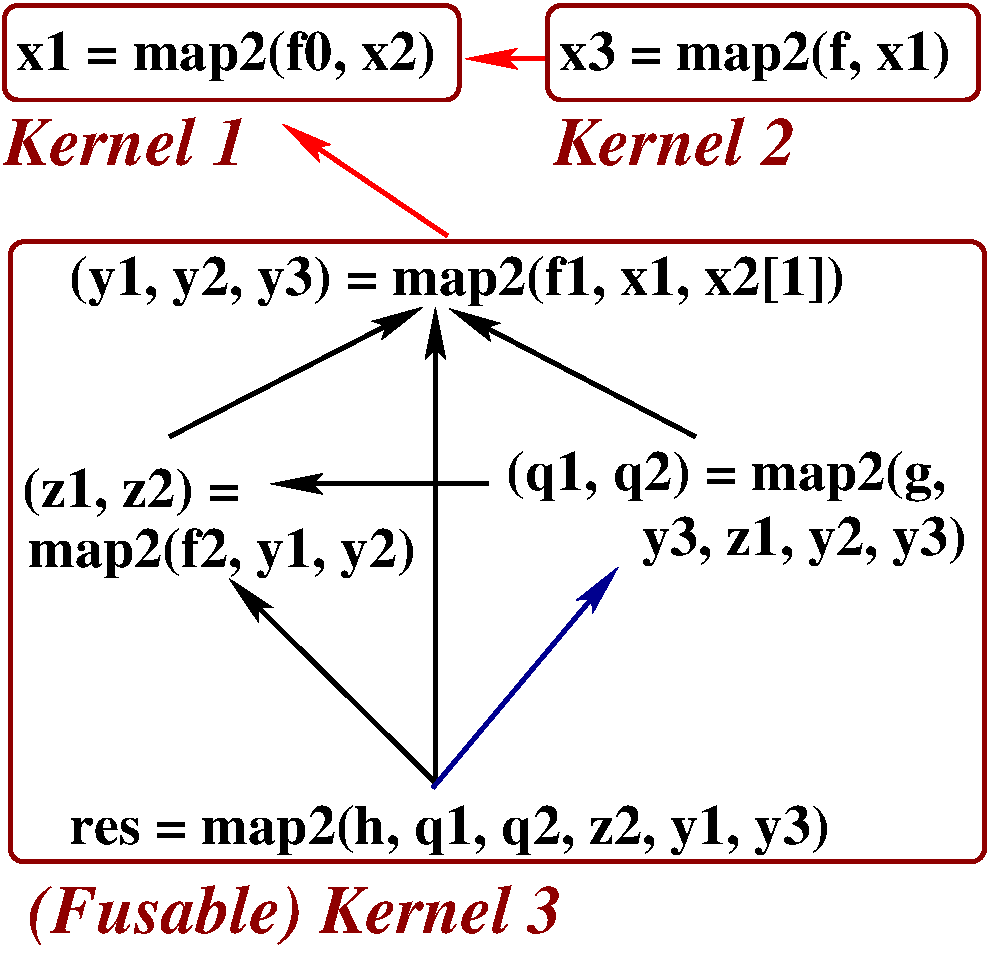
\includegraphics[height=19ex]{Figures/T1T2} \hspace{2ex} 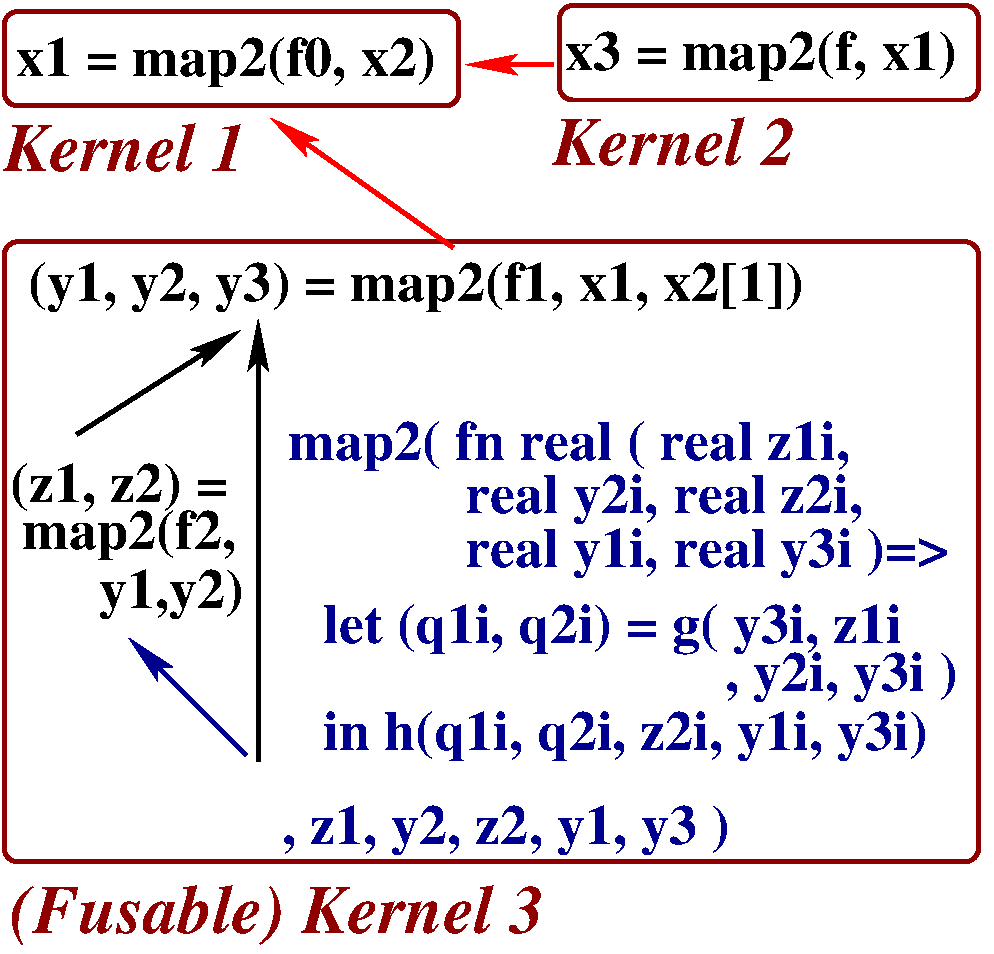
\includegraphics[height=19ex]{Figures/T1T2Fuse1} \hspace{2ex}
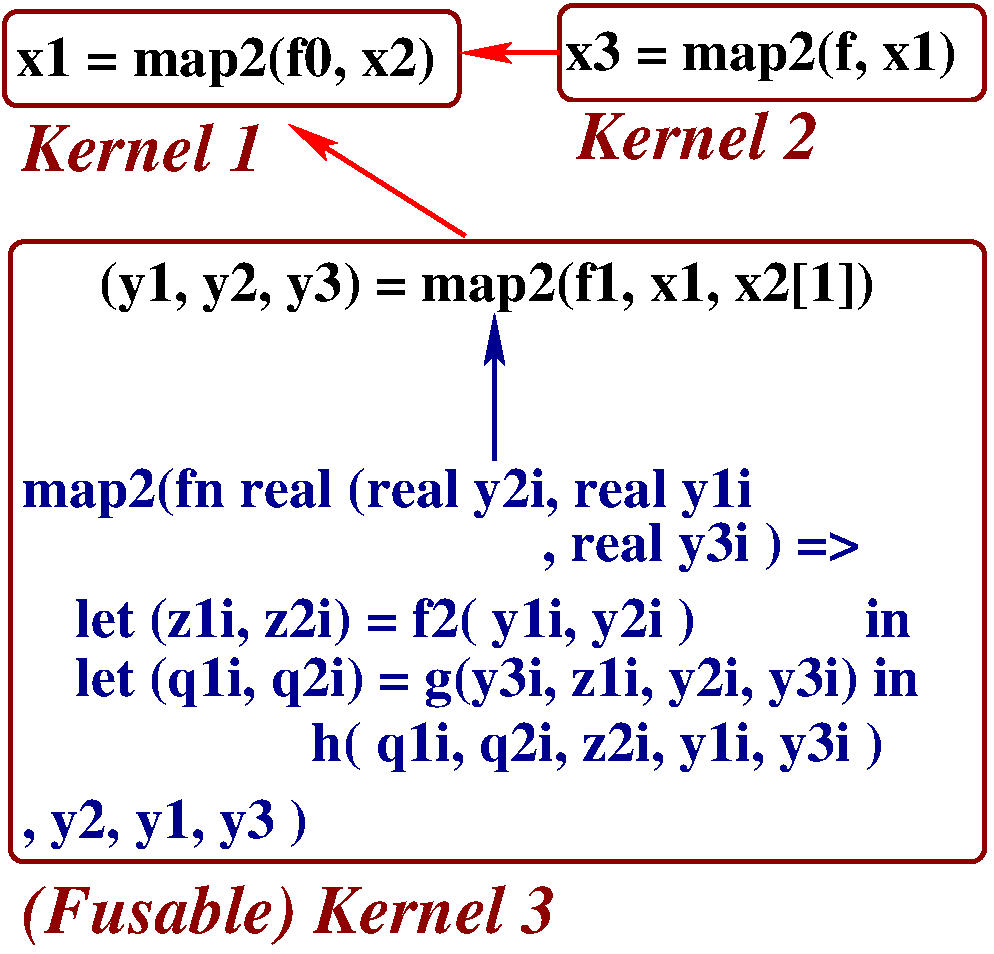
\includegraphics[height=19ex]{Figures/T1T2Fuse2} %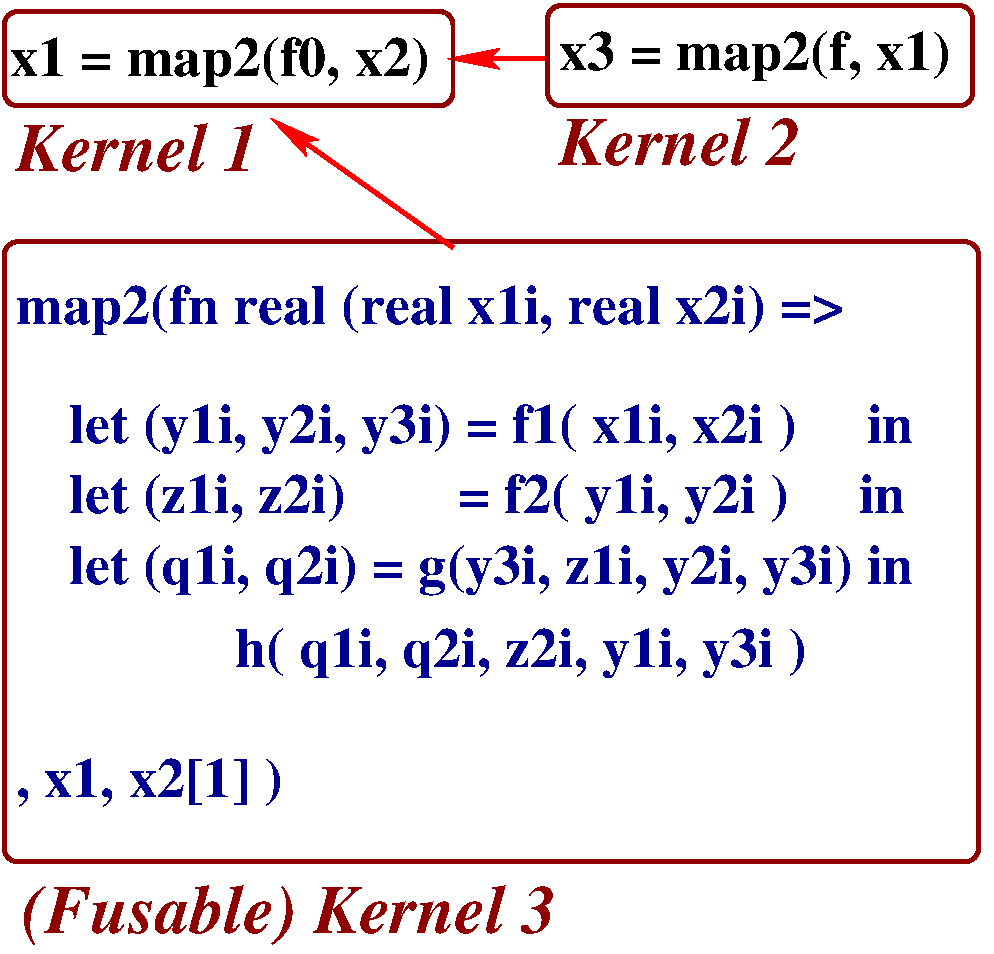
\includegraphics[height=17ex]{Figures/T1T2Fuse3}
\end{frame}


\subsection{Simple/Enabling Optimizations}

\begin{frame}[fragile,t]
    \frametitle{Example of Simple Optimizations}

\emp{\bf Liveness analysis \& Register allocation}: compiler course.

\bigskip

\emp{\bf Common-Subexpression Elimination (CSE)}: if the same expression
$e$ is computed twice, replace if possible the second occurrence of $e$
with the temporary that holds the value of the first computation of $e$.

\bigskip

\emp{\bf Copy Propagation (CP)}: after a statement {\tt x~:=~y}, 
we know that {\tt x} and {\tt y} have the same value, hence we can replace 
all occurrences of {\tt x} with {\tt y} between this assignment and the next 
definition of {\tt x} or {\tt y}.

\bigskip

\emp{\bf Dead-Code Elimination (DC)} (one reason is copy propagation):
\begin{itemize}
    \item can safely remove any statement that defines a dead variable,
    \item a branch to dead code moved to whatever follows the dead code,
    \item if a branch-condition value is statically known $\Leftrightarrow$ merge two BBs.
\end{itemize}

\bigskip

\emp{\bf Constant Folding and Propagation (CtF/P)}: if possible,
expressions should be computed at compile time, and the constant
result should be propagated. {\bf And these are just a few!}


\end{frame}

\begin{frame}[fragile,t]
    \frametitle{Example: Common-Subexpression Elimination
                    (CSE) and Copy Propagation (CP)}

Shown at basic-block level, but {\em Data-flow} analysis extends it on CFG.

\begin{block}{Original{\tt~~~~~~~}After CSE1{\tt~~~~~~}After CP1{\tt~~~}After CSE2 \& CP2}
\begin{columns}
\column{0.18\textwidth}
\begin{colorcode}[fontsize=\scriptsize]
t1 := 4  - 2
t2 := t1 / 2
t3 := a  * t2
t4 := \emp{t3 * t1}
t5 := t4 + b
t6 := \emp{t3 * t1}
t7 := t6 + b
c  := t5 * t7
\end{colorcode} 
\column{0.22\textwidth}
\begin{colorcode}[fontsize=\scriptsize]
t1 := 4  - 2
t2 := t1 / 2
t3 := a  * t2
t4 := t3 * t1
t5 := t4 + b
\emp{t6} := \green{t4}
t7 := \emp{t6} + b
c  := t5 * t7
\end{colorcode} 
\column{0.22\textwidth}
\begin{colorcode}[fontsize=\scriptsize]
t1 := 4  - 2
t2 := t1 / 2
t3 := a  * t2
t4 := t3 * t1
\green{t5} := \emp{t4 + b}
t6 := t4
t7 := \emp{t4 + b}
c  := t5 * t7
\end{colorcode} 
\column{0.22\textwidth}
\begin{colorcode}[fontsize=\scriptsize]
t1 := 4  - 2
t2 := t1 / 2
t3 := a  * t2
t4 := t3 * t1
t5 := \emp{t4 + b}
t6 := t4
t7 := t5
c  := t5 * \green{t5}
\end{colorcode} 
\end{columns}
\end{block}

\bigskip

Copy propagation makes further common-subexpression elimination
possible and the reverse.

\end{frame}


\begin{frame}[fragile,t]
    \frametitle{Example Continuation: Constant Folding (CFP) \&
                    Copy Propagation (CP) \& Dead Code Elim (DCE)}

Shown at basic-block level, but {\em Data-flow} analysis extends it on CFG.

\begin{block}{Original{\tt~~~~~~}After CtFP{\tt~~~~~~~}After CP{\tt~~~~~~~~}After DCE}
\begin{columns}
\column{0.18\textwidth}
\begin{colorcode}[fontsize=\scriptsize]
\emp{t1 := 4  - 2}
\emp{t2 := t1 / 2}
t3 := a  * \emp{t2}
t4 := t3 * \emp{t1}
t5 := t4 + b
t6 := t4
t7 := t5
c  := t5 * t5
\end{colorcode} 
\column{0.22\textwidth}
\begin{colorcode}[fontsize=\scriptsize]
t1 := 2
t2 := 1
\emp{t3 := a}
t4 := \emp{t3} * 2
t5 := t4 + b
t6 := t4
t7 := t5
c  := t5 * t5
\end{colorcode} 
\column{0.22\textwidth}
\begin{colorcode}[fontsize=\scriptsize]
\emp{t1 := 2}
\emp{t2 := 1}
\emp{t3 := a}
t4 := a  * 2
t5 := t4 + b
\emp{t6 := t4}
\emp{t7 := t5}
c  := t5 * t5
\end{colorcode} 
\column{0.22\textwidth}
\begin{colorcode}[fontsize=\scriptsize]



t4 := a  * 2
t5 := t4 + b


c  := t5 * t5
\end{colorcode} 
\end{columns}
\end{block}

\bigskip

Very useful in optimizing the critical-execution path or eliminating
the redundancies introduced by various transformations 
(by the compiler).

\end{frame}

\end{document}
